%%%%%%%%%%%%%%%%%%%%%%%%%%%%%%%%%%%%%%%%%
% Oliver Lemon made minor edits (jan 2015)  to : 
% Masters/Doctoral Thesis 
% LaTeX Template
% Version 1.43 (17/5/14)
%
% This template has been downloaded from:
% http://www.LaTeXTemplates.com
%
% Original authors:
% Steven Gunn 
% http://users.ecs.soton.ac.uk/srg/softwaretools/document/templates/
% and
% Sunil Patel
% http://www.sunilpatel.co.uk/thesis-template/
%
% License:
% CC BY-NC-SA 3.0 (http://creativecommons.org/licenses/by-nc-sa/3.0/)
%
% Note:
% Make sure to edit document variables in the Thesis.cls file
%
%%%%%%%%%%%%%%%%%%%%%%%%%%%%%%%%%%%%%%%%%

%----------------------------------------------------------------------------------------
%	PACKAGES AND OTHER DOCUMENT CONFIGURATIONS
%----------------------------------------------------------------------------------------

\documentclass[10pt, oneside, article]{Thesis} % The default font size and one-sided printing (no margin offsets)

\graphicspath{{Pictures/}} % Specifies the directory where pictures are stored
\usepackage{ragged2e}
\usepackage[square,numbers]{natbib}
\bibliographystyle{unsrtnat}
\renewcommand{\bibname}{References}
% --- Hyperref setup ---
\usepackage{pgfplots}
\usepackage{pgfplotstable}
\usepackage{filecontents}
\hypersetup{urlcolor=blue, colorlinks=true} % Colors hyperlinks in blue - change to black if annoying
\usepackage{graphicx}
\usepackage{amsmath}
\usepackage{tikz}
\usepackage{pgfplots}
\pgfplotsset{compat=1.17}
\usepackage{algorithm}
\usepackage{algorithmic}
\usepackage{hyperref}
\usepackage{subcaption}
\usepackage{tikz}
\usetikzlibrary{positioning, shapes, arrows.meta}
\usepackage[dvipsnames]{xcolor}
\usepackage{titlesec}
\usepackage{float}
\usepackage{longtable}
\usepackage{datetime}
\usepackage{multirow}

\titleformat*{\section}{\huge\bfseries}
\titleformat*{\subsection}{\LARGE\bfseries}
\titleformat*{\subsubsection}{\Large\bfseries}
\titleformat*{\paragraph}{\Large\bfseries}
\titleformat*{\subparagraph}{\large\bfseries}

\title{Detection of Primary User Emulation
Attack in Cognitive Radio Network:
Clustering Algorithm} % BUT you should use use " \title{\ttitle} " here instead to define the thesis title ! 
% \ttitle is defined in the file Thesis.cls 

\newcommand{\vect}[1]{\mathbf{#1}}
\newcommand{\mat}[1]{\mathbf{#1}}
\usepackage[en-IN]{datetime2}


\begin{document}
% \definecolor{bluegreen}{rgb}{0.0, 0.87, 0.87} % Define bluegreen color
\usetikzlibrary{shapes.geometric, arrows, positioning, fit}

\tikzstyle{process} = [rectangle, minimum width=3cm, minimum height=1cm, text centered, draw=black, fill=blue!10]
\tikzstyle{decision} = [diamond, minimum width=3cm, minimum height=1cm, text centered, draw=black, fill=green!10]
\tikzstyle{cluster} = [rectangle, minimum width=2.5cm, minimum height=1cm, text centered, draw=black, fill=yellow!20]
\tikzstyle{parallel} = [rectangle, minimum width=2.5cm, minimum height=1cm, text centered, draw=black, fill=orange!20]
\tikzstyle{evaluation} = [rectangle, minimum width=3cm, minimum height=1cm, text centered, draw=black, fill=red!10]
\tikzstyle{arrow} = [thick,->,>=stealth]

\frontmatter % Use roman page numbering style (i, ii, iii, iv...) for the pre-content pages

\setstretch{1.3} % Line spacing of 1.3

% Define the page headers using the FancyHdr package and set up for one-sided printing
% \fancyhead{} % Clears all page headers and footers
% \rhead{\thepage} % Sets the right side header to show the page number
% \lhead{} % Clears the left side page header
\fancyhf{} % Clear all headers and footers

% Page number on the outer side (right on odd, left on even pages)
\fancyhead[RO,LE]{\thepage}

% Chapter title on the inner side
\fancyhead[LO,RE]{\nouppercase{\leftmark}}


\pagestyle{fancy} % Finally, use the "fancy" page style to implement the FancyHdr headers

\newcommand{\HRule}{\rule{\linewidth}{0.5mm}} % New command to make the lines in the title page

% PDF meta-data
\hypersetup{pdftitle={\ttitle}}
\hypersetup{pdfsubject=\subjectname}
\hypersetup{pdfauthor=\authornames}
\hypersetup{pdfkeywords=\keywordnames}

%----------------------------------------------------------------------------------------
%	TITLE PAGE
%----------------------------------------------------------------------------------------

\begin{titlepage}
\vspace{-1cm}
\begin{center}
{\scshape\LARGE ASSAM UNIVERSITY \par}\vspace{0cm}

\HRule \\[0.4cm] % Horizontal line
{\huge \bfseries Detection of Primary User Emulation
Attack in Cognitive Radio Network: Clustering Algorithm}\\[.1cm] % Thesis title
\HRule \\[1.5cm] % Horizontal line
\vspace{-.8cm}
\large \textit{A report submitted in partial fulfilment of the requirements for the degree of \\ \textbf{\degreename}}\\[0.3cm] % University requirement text
\vspace{-.4cm}\textit{in }\\ \textbf{Computer Science and Engineering}

 
\begin{minipage}[t]{0.8\textwidth}
\begin{center}
  \textbf{Submitted By:}\\
Rishav Raj \\ Reg. No. : 20210020996\hspace{10pt}   of 2021-22\\
Snehasish Das\\ Reg. No. : 20210000157\hspace{10pt} of 2021-22\\
Sumir Das \\ Reg. No. : 20220015756\hspace{10pt}   of 2021-22\\
Debraj Dutta Gupta\\ Reg. No. : 20200014383\hspace{10pt} of 2021-22
\end{center} \large


\end{minipage}
\\[0.8cm]
\begin{minipage}[t]{0.8\textwidth}
\begin{center} \large
\textbf{Under the Supervision of:} \\
{\supname}\\
Assistant Professor, Department of Computer Science and Engineering
 %\\ Supervisor name - remove the \href bracket to remove the link  
\end{center}
\end{minipage}\\[1.5cm]
 

{

\includegraphics[width=3cm]{Logo.png} \\% University/department logo - uncomment to place it
Triguna Sen School of Tehnology\\ 
Department of Computer Science and Engineering\\ % Research group name and department name
Assam University, Silchar 788011 \\
\large July 12, 2025}\\[1cm]%\today}\\[1cm] % Date
\end{center}

\end{titlepage}

%----------------------------------------------------------------------------------------
%	DECLARATION PAGE
%	Your institution may give you a different text to place here
%----------------------------------------------------------------------------------------
\begin{center}
    
\includegraphics[width=4cm]{Logo.png} % University/department logo - uncomment to place it
 

\end{center}
\Declaration{

\addtocontents{toc}{\vspace{1em}} % Add a gap in the Contents, for aesthetics



We, the undersigned, declare that this report titled 'Detection of Primary User Emulation Attack in Cognitive Radio Network: Clustering Algorithm' and the work presented in this report is our own. We confirm that this work submitted for assessment is our own and is expressed in our own words. Any uses made within it of the works of  other authors in any form (e.g., ideas, equations, figures, text,  tables, programs) are properly acknowledged at any point of their  use . To the best of our knowledge and belief, the same report has not been submitted either by us or by any other person for the award of any other degree or diploma of the University or other
institute of higher learning.

 \vspace{2cm} 
\textbf{Rishav Raj (20210020996)}\\
\rule[1em]{40em}{0.5pt}\\ % This prints a line for the signature
\textbf{Snehasish Das (20210000157)}\\
\rule[1em]{40em}{0.5pt}\\
\textbf{Sumir Das (20220015756)}\\
\rule[1em]{40em}{0.5pt}\\
\textbf{Debraj Dutta Gupta (20200014383)}\\
\rule[1em]{40em}{0.5pt}\\
Date:\\
\rule[1em]{20em}{0.5pt}\\ % This prints a line to write the date
Place:\\
\rule[1em]{20em}{0.5pt}\\
}

\clearpage % Start a new page

%-------------------------------------------------------------------------------

%-------------------------------------------------------------------------------
% CERTIFICATE PAGE
%
% Use the \Certificate command to print the Certificate in the document
%-------------------------------------------------------------------------------

\begin{center}

\includegraphics[width=3cm]{Logo.png}\\ % University/department logo - uncomment to place it
Department of Computer Science and Engineering \\
Assam University, Silchar-788011\\
\Certificate{
This is to certify that the report entitled \\ \textit{Detection of Primary User Emulation
Attack in Cognitive Radio Network:
Clustering Algorithm}} \\  submitted by \\ \textit{\textbf{Rishav Raj,\\ Snehasish Das,\\ Sumir Das, \\ Debraj Dutta Gupta}} \\ to the Department of Computer Science and Engineering, Assam University, Silchar in partial fulfilment of the requirements for the the award of the Degree of\\ \textbf{Bachelor of Technology} \\ in \\ \textbf{Computer Science and Engineering} \\ is a bonafide record of the work carried out by them under my supervision. It is further certified that the candidates have complied with all the formalities as per the requirements of Assam University.\\ \vspace{2cm}


\begin{flushleft}
 \rule[1em]{30em}{0.5pt}\\  \textbf{Name \& Signature (Supervisor)}  \\ \vspace{1cm}
 \rule[1em]{30em}{0.5pt}\\ \textbf{Prof. Sudipta Roy (Head of the Department)}  \\ \vspace{1cm}
\rule[1em]{30em}{0.5pt}\\ \textbf{External Examiner's Name \& Signature}  \\
\begin{flushright}
Date and Seal
\end{flushright}
\end{flushleft} \large

\end{center}
\clearpage


%-------------  ---------------------------------------------------------------------------
%	ACKNOWLEDGEMENTS
%----------------------------------------------------------------------------------------

\setstretch{1.3} % Reset the line-spacing to 1.3 for body text (if it has changed)

\acknowledgements{\addtocontents{toc}{\vspace{1em}} % Add a gap in the Contents, for aesthetics

We would like to express our sincere gratitude to our Head of Department, \textbf{Dr. Tapodhir Acharjee} from the Department of Computer Science and Engineering and especially to our Project guide, \textbf{Dr. Wangjam Niranjan Singh}, for his invaluable guidance and support throughout this research project. \\ \\
We express our appreciation to the entire team. Our collaboration and willingness to share
knowledge and experiences has been invaluable to us.
Our constructive criticism and input has helped us refine our ideas and clarify our arguments.
We are truly grateful to have such a supportive academic team.\\

\begin{flushright}
    
    Team:-
    \\Rishav Raj\\Snehasish Das\\Sumir Das\\Debraj Dutta Gupta\\
\end{flushright}
}
\clearpage % Start a new page
%----------------------------------------------------------------------------------------
%	ABSTRACT PAGE
%----------------------------------------------------------------------------------------

\addtotoc{Abstract} % Add the "Abstract" page entry to the Contents

%\abstract{\addtocontents{toc}{\vspace{1em}} % Add a gap in the Contents, for aesthetics

 {\huge{\textit{Abstract}} \par}{\addtocontents{toc}{\vspace{1em}} 

Cognitive Radio Networks (CRNs) have emerged as an intelligent solution to spectrum scarcity; however, they are highly vulnerable to Primary User Emulation Attacks (PUEAs), where malicious users mimic legitimate signals to disrupt communication. Existing detection methods often fail to adapt across diverse network layouts and attack intensities, limiting their effectiveness. This thesis presents an integrated detection framework that combines enhanced clustering techniques (K-means, Spectral, and Agglomerative) with advanced distance-based classification methods (KNN and Means enhancement). A key innovation is the automatic parameter optimization enabling robust adaptability to varying operating conditions, with enhanced variants significantly outperforming baseline implementations. The framework was validated through extensive simulations across 75 network topologies, three distance scenarios (100, 65, and 30 units), and five PUEA penetration levels (10–50\%), with 30 secondary users operating over 400 time slots. Detection was based on Manhattan distance matrices derived from five statistical signal features. Results demonstrate exceptional performance with enhanced K-means variants achieving superior detection: K-means KNN achieved 91.54\% detection rate with 6.84\% false detection, and K-means Means achieved 91.48\% detection rate with 6.83\% false detection, both outperforming the original K-means (91.36\% detection, 6.92\% false detection). Enhanced Spectral KNN achieved 66.02\% detection rate compared to Enhanced Spectral Original's 61.60\%, while Enhanced Agglomerative KNN achieved 62.69\% detection rate surpassing Enhanced Agglomerative Original's 58.27\%. Distance analysis revealed optimal performance in close proximity scenarios (91.54\% detection rate) compared to far distance scenarios (85.43\% detection rate), representing a 6.11 percentage point improvement. These enhanced detection capabilities significantly surpass the 60–75\% detection rates reported in prior literature, establishing enhanced K-means variants as the new benchmark methods for PUEA detection and contributing a scalable, adaptable solution to CRN security.
}


\clearpage % Start a new page

%----------------------------------------------------------------------------------------
%	LIST OF CONTENTS/FIGURES/TABLES PAGES
%----------------------------------------------------------------------------------------

\pagestyle{fancy} % The page style headers have been "empty" all this time, now use the "fancy" headers as defined before to bring them back

\lhead{\emph{Contents}} % Set the left side page header to "Contents"
\tableofcontents % Write out the Table of Contents

\lhead{\emph{List of Tables}} % Set the left side page header to "List of Tables"
\listoftables % Write out the List of Tables

\lhead{\emph{List of Figures}} % Set the left side page header to "List of Figures"
\listoffigures % Write out the List of Figures


%----------------------------------------------------------------------------------------
%	ABBREVIATIONS
%----------------------------------------------------------------------------------------

\clearpage % Start a new page

\setstretch{1.5} % Set the line spacing to 1.5, this makes the following tables easier to read

\lhead{\emph{Abbreviations}} % Set the left side page header to "Abbreviations"


\listofsymbols{ll} % Two-column format: Symbol and Description
{
\textbf{CRN}  & Cognitive Radio Network \\
\textbf{PUEA} & Primary User Emulation Attack \\
\textbf{PU}   & Primary User \\
\textbf{SU}   & Secondary User \\
\textbf{ML}   & Machine Learning \\
\textbf{DSA}  & Dynamic Spectrum Access \\
\textbf{SNR}  & Signal-to-Noise Ratio \\
\textbf{ROC}  & Receiver Operating Characteristic \\
\textbf{AUC}  & Area Under Curve \\
\textbf{ARI}  & Adjusted Rand Index \\
\textbf{KNN}  & K-Nearest Neighbors \\
\textbf{CSV}  & Comma-Separated Values \\
\textbf{RSS}  & Received Signal Strength \\
\textbf{AWGN} & Additive White Gaussian Noise \\
}


%----------------------------------------------------------------------------------------
%	PHYSICAL CONSTANTS/OTHER DEFINITIONS
%----------------------------------------------------------------------------------------

%\clearpage % Start a new page


%----------------------------------------------------------------------------------------
%	SYMBOLS
%----------------------------------------------------------------------------------------

\clearpage % Start a new page

\lhead{\emph{Symbols}} % Set the left side page header to "Symbols"


\addcontentsline{toc}{chapter}{List of Symbols}
\lhead{\emph{List of Symbols}} % Optional header

\listofnomenclature{lll} % Symbol, Description, Unit
{
$P_d$ & Probability of detection & -- \\
$P_f$ & Probability of false alarm & -- \\
$\gamma$ & Received signal power & $dBm$ \\
$\sigma^2$ & Noise variance & dB \\
$\lambda$ & Decision threshold & dB \\
$d_{ij}$ & Distance between points $i$ and $j$ & Units \\
$\sigma$ & Spectral clustering affinity (RBF) kernel width & Units \\
$k$ & Number of clusters & -- \\
$\vect{x}$ & Feature vector & -- \\
$\mat{D}$ & Distance matrix & -- \\
$N$ & Number of data points & -- \\
$\mu$ & Cluster centroid & -- \\

}

%----------------------------------------------------------------------------------------
%	DEDICATION
%----------------------------------------------------------------------------------------

% \setstretch{1.3} % Return the line spacing back to 1.3

% \pagestyle{empty} % Page style needs to be empty for this page

% % \dedicatory{For/Dedicated to/To my\ldots} % Dedication text

% \addtocontents{toc}{\vspace{2em}} % Add a gap in the Contents, for aesthetics

%----------------------------------------------------------------------------------------
%	THESIS CONTENT - CHAPTERS
%----------------------------------------------------------------------------------------

\mainmatter % Begin numeric (1,2,3...) page numbering

\pagestyle{fancy} % Return the page headers back to the "fancy" style

% Include the chapters of the thesis as separate files from the Chapters folder
% Uncomment the lines as you write the chapters

% Chapter 1

\chapter{Introduction} % Main chapter title

\label{Chapter1} % For referencing the chapter elsewhere, use \ref{Chapter1} 

\lhead{Chapter 1. \emph{Introduction}} % Change X to a consecutive number; this is for the header on each page - perhaps a shortened title

%----------------------------------------------------------------------------------------
\section{\textbf{Wireless Applications}}

Our modern society heavily depends on the wireless spectrum for communication purposes.
Telecommunications, financial transactions, health services, military services, environment
surveillance, entertainment, and social activities are just several of the numerous applications
examples in our daily life.
\begin{figure}
    \centering
    \includegraphics[width=1\linewidth]{Figures/chapter1/Forecast year-on-year mobile data traffic growth rates by region 2022–2029.png}
    \caption{Forecast year-on-year mobile data traffic growth rates by region 2022–2029 \cite{ref26}}
    \label{fig:forecast1}
\end{figure}

Forecast year-on-year growth rates of mobile data traffic. The growth rate for mobile data is expected to slow every year between 2022 and 2029 in all regions. The region, which includes India, Nepal and Bhutan, consistently shows a higher growth rate than the global average.
All lines are trending downwards, indicating that while data usage is still growing, it is growing at a slower pace each year (Figure: \ref{fig:forecast1}).  

\begin{figure}
    \centering
    \includegraphics[width=1\linewidth]{Figures/chapter1/Forecast yearly net added mobile data traffic 2022–2029.png}
    \caption{Forecast yearly net added mobile data traffic 2022–2029 \cite{ref26}}
    \label{fig:forecast2}
\end{figure}

 Forecast yearly net added mobile data traffic.The total amount of new mobile data traffic added each year is forecast to increase steadily from 2022 to a peak in 2027. After 2027, the amount of newly added traffic is expected to decrease slightly. The bars get taller until 2027, meaning that the sheer volume of new data added to networks will continue to grow for the next few years (Figure: \ref{fig:forecast2}).

\section{\textbf{Cognitive Radio Network(CRN)}}
With the rapid development in communication applications the spectrum becomes more congested and also the need for data rate increased. The radio spectrum is a limited resource and the service is allocated by fixed spectrum assignment. So some frequencies are heavily used, and other bands are weakly used.
The number of devices that use unlicensed spectrum is growing, which indicates an increase in spectrum demand. So spectrum scarcity is a major issue faced by wireless networks. In order to overcome this issue, dynamic spectrum access (DSA) is introduced, which improves the spectrum efficiency. In DSA the unlicensed systems are allowed to use the licensed bands without interfering with the existing user. So the weakly used spectrum can be used by other users. In Figure:\ref{fig:crn} Cognitive Radio (CR)
uses dynamics spectrum allocation which provides higher bandwidth and efficient spectrum usage. CR enables reuse of the licensed spectrum in an unlicensed manner i.e., it opens the licensed bands to unlicensed users to use them without causing any interference to the licensed user. Radio sensing, self adaptation and dynamic spectrum sharing are the abilities of CR. Spectrum under utilization and spectrum scarcity can be mitigated by an efficient spectrum usage of CR \cite{ref2}. 

Key features of Cognitive Radio include:
    Radio Sensing,
    Self-Adaptation
    and Dynamic Spectrum Sharing




\subsection{\textbf{Overview of CR and CRN}}

CR stands for Cognitive Radio and CRN stands for Cognitive Radio Networks \cite{ref1}. These are advanced wireless communication technologies that aim to improve spectrum utilization and efficiency.

\textbf{Cognitive Radio (CR)}

    A radio that can intelligently sense its environment, detect available spectrum opportunities, and dynamically adapt its parameters (e.g., frequency, power, modulation) to efficiently utilize the spectrum.
    Key features are 
        Spectrum Sensing: The ability to detect unused or underutilized spectrum bands.
        Spectrum Decision: The ability to make intelligent decisions about which spectrum bands to use.
        Spectrum Access: The ability to dynamically access and utilize available spectrum bands.
    Benefits are  
        Improved spectrum utilization, Reduced interference, Increased network capacity, Enhanced flexibility and adaptability. \\ 

\textbf{Cognitive Radio Networks (CRN)}

\begin{figure}
    \centering
    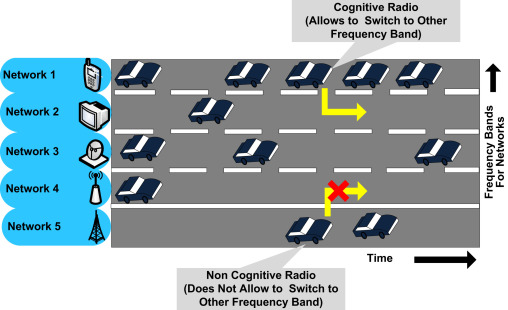
\includegraphics[width=0.8\linewidth]{Figures/chapter1/CRN overview.jpg}
    \caption{CRN overview \cite{ref27}}
    \label{fig:crn}
\end{figure}

A network of cognitive radios that can collaborate and coordinate their spectrum access to optimize overall network performance.
    Key features \cite{ref1} are Cooperative Spectrum Sensing: Multiple cognitive radios can collaborate to improve spectrum sensing accuracy and coverage.
        Spectrum Sharing: Cognitive radios can share spectrum resources among themselves and with other networks.
        Dynamic Spectrum Management: CRNs can dynamically manage spectrum access to optimize network performance and meet changing demands.
    Benefits are : Improved spectrum efficiency, Enhanced network reliability, Increased network capacity and Better quality of service
 
\subsection{\textbf{Functions of CRN}}

Cognitive Radio Networks (CRNs) leverage advanced technologies to optimize the use of the radio frequency (RF) spectrum, addressing the challenges of spectrum scarcity and inefficiency through several key functional areas \cite{ref1}. The foundational function is spectrum sensing, which enables cognitive radios to detect unused portions of the spectrum, often referred to as spectrum holes or white spaces, allowing them to identify which channels are occupied by primary users and which are available for secondary users \cite{ref1,ref6}. Various sophisticated techniques are employed for spectrum sensing, including energy detection, matched filtering, and cyclostationary feature detection, each offering distinct advantages and limitations \cite{ref4,ref6}. Once available spectrum is identified, spectrum management becomes crucial as cognitive radios must effectively select the best available channel based on communication requirements such as bandwidth, signal quality, and interference levels, ensuring dynamic adaptation to changing network conditions and user demands \cite{ref1,ref3}.

The operational capabilities of CRNs are further enhanced by spectrum mobility and sharing functions, which are essential for maintaining service quality while adhering to regulatory constraints. Since cognitive radios operate as secondary users with lower priority, spectrum mobility enables them to seamlessly transition to alternative available channels when primary users are detected, maintaining ongoing communications without disruption \cite{ref1,ref3}. In multi-user environments, spectrum sharing coordinates access among various cognitive radios to ensure fair usage and minimize interference through sophisticated scheduling algorithms and protocols \cite{ref1,ref3}. The cognitive capability encompasses the fundamental ability to perceive, learn, and adapt to environmental changes, enabling informed decision-making for channel selection and usage \cite{ref1,ref2}. Additionally, reconfigurability allows cognitive radios to dynamically adjust transmission parameters such as frequency, power, and modulation schemes based on detected spectrum conditions, while learning and adaptation capabilities enable performance enhancement over time through experience-based strategy optimization and historical data analysis \cite{ref1,ref3,ref9,ref19}. These functions collectively enable CRNs to utilize the RF spectrum more efficiently, improving overall communication quality and expanding network capacity to support growing numbers of connected devices and applications \cite{ref1,ref2,ref3}.


\subsection{\textbf{Cognitive cycle}}

The cognitive cycle is a fundamental concept in Cognitive Radio Networks (CRNs), representing the iterative process through which cognitive radios (CRs) adaptively manage spectrum resources as illustrated in Figure \ref{fig:cr_cycle} \cite{ref1,ref3}. This comprehensive cycle consists of four interconnected key functions that work together to enable intelligent spectrum management. The initial phase, spectrum sensing, involves continuous monitoring of the radio environment to detect the presence of primary users (PUs) and identify available spectrum bands, which is crucial for avoiding interference with licensed users and ensuring efficient spectrum utilization \cite{ref1,ref4,ref6}. Following the sensing phase, spectrum decision requires cognitive radios to analyze the sensed data and make intelligent choices about which spectrum band to utilize, considering factors such as channel quality, secondary user requirements, and potential interference levels \cite{ref1,ref3}.

\begin{figure}
    \centering
    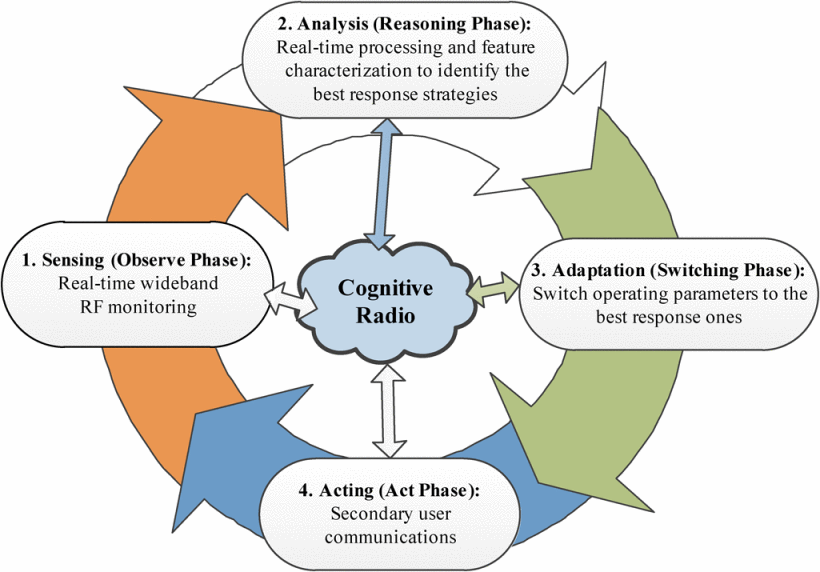
\includegraphics[width=0.8\linewidth]{Figures/chapter1/cr_cycle.png}
    \caption{Cognitive Cycle \cite{ref29}}
    \label{fig:cr_cycle}
\end{figure}

The operational phases of the cognitive cycle ensure seamless spectrum access and dynamic adaptation to changing radio environments. Once a spectrum decision is made, spectrum sharing becomes essential as cognitive radios must negotiate access to the selected spectrum band through coordination with other cognitive radios, ensuring spectrum utilization without causing disruption to primary users or other secondary users \cite{ref1,ref3}. The final phase, spectrum mobility, enables cognitive radios to dynamically switch channels as the radio environment changes, allowing them to maintain communication links while avoiding interference with primary users that may become active \cite{ref1,ref3}. This iterative cognitive cycle enables CRs to continuously adapt to the dynamic nature of wireless communication, optimizing spectrum usage and enhancing overall network performance through intelligent, real-time decision-making processes \cite{ref1,ref3}.

%----------------------------------------------------------------------------------------
\section{\textbf{Architecture of CRN}}

The architecture of Cognitive Radio Networks (CRNs) is designed to facilitate intelligent spectrum management and enhance communication efficiency through a sophisticated framework of interconnected components \cite{ref1,ref2}. As illustrated in Figure \ref{fig:CRN_arc}, the core of this architecture is the cognitive engine, which serves as the brain of the CR, processing environmental information and making intelligent decisions based on the cognitive cycle \cite{ref1}. This cognitive engine incorporates advanced machine learning algorithms to continuously improve its decision-making capabilities over time, enabling adaptive and intelligent spectrum management \cite{ref9,ref19}. The spectrum sensing module works in conjunction with the cognitive engine to detect the presence of primary users and identify idle channels through various sophisticated techniques, including energy detection, matched filtering, and cyclostationary feature detection, ensuring accurate spectrum awareness \cite{ref4,ref6,ref11}.

\begin{figure}[ht]
    \centering
    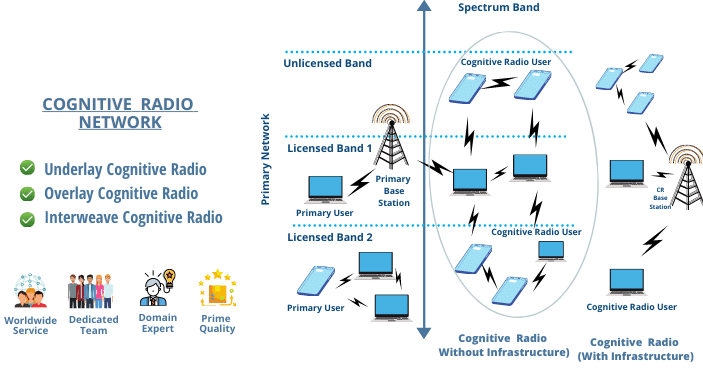
\includegraphics[width=\linewidth]{Figures/chapter1/CRN-Thesis.png}
    \caption{CRN Environment \cite{ref28}}
    \label{fig:CRN_arc}
\end{figure}

The operational efficiency of CRNs is further enhanced by the spectrum management module, which allocates spectrum resources based on user demands and environmental conditions while ensuring efficient utilization that balances the needs of both primary and secondary users \cite{ref1,ref3}. The communication module facilitates reliable data transmission over the selected spectrum, ensuring efficient communication between devices throughout the network \cite{ref2}. Given the inherent vulnerabilities of CRNs to various security threats, a robust security framework is integrated into the architecture as an essential component, incorporating mechanisms for detecting and mitigating attacks such as Primary User Emulation Attacks (PUEA) and Spectrum Sensing Data Falsification (SSDF) \cite{ref1,ref7,ref25}. Overall, this comprehensive architecture enables CRNs to support dynamic spectrum access while maintaining reliable communication and robust security measures \cite{ref1,ref25}.

%----------------------------------------------------------------------------------------
\section{\textbf{Security Issues in CRN}}

Cognitive Radio Networks (CRNs), while designed to address spectrum scarcity through dynamic spectrum access, introduce significant security vulnerabilities that can severely impact network performance and reliability \cite{ref25}. The most critical threat is the Primary User Emulation Attack (PUEA), where malicious users mimic the behavior of primary users, forcing legitimate secondary users to vacate spectrum bands and leading to inefficient spectrum utilization \cite{ref7}. This attack essentially functions as a denial of service mechanism, causing secondary users to experience increased call drop rates, communication delays, and severe quality of service degradation \cite{ref1}. Additionally, Spectrum Sensing Data Falsification (SSDF) attacks exploit vulnerabilities in collaborative spectrum sensing by manipulating sensing data to mislead secondary users about spectrum availability, further compromising network integrity \cite{ref6}.

The dynamic nature of CRNs creates additional security challenges that extend beyond traditional wireless network threats. Control channel vulnerabilities pose particular risks, as compromise of the common control channel (CCC) used for exchanging control messages can lead to complete network outages, rendering entire CRN systems inoperable \cite{ref25}. The continuous requirement for secondary users to estimate primary user parameters during dynamic spectrum access exposes them to eavesdropping and other sophisticated attacks \cite{ref3}. These security issues can be broadly categorized into infrastructure-based attacks (such as PUEA and SSDF) and infrastructure-less attacks (including greedy secondary user behaviors), each presenting unique challenges that require comprehensive security frameworks to ensure reliable and secure cognitive radio operations \cite{ref1,ref7}.

\chapter{Background}
\label{Chapter2}
\lhead{Chapter 2. \emph{Background}} % Change X to a consecutive number; this is for the\b\subsection{L\beLocation ve\begin{figure}
\section{\textbf{Dynamic Spectrum Access}}

Dynamic Spectrum Access (DSA) represents a paradigm shift from traditional static spectrum allocation to more flexible and efficient spectrum utilization strategies. Akyildiz et al. \cite{ref3} established the foundational framework for next generation dynamic spectrum access networks, highlighting how DSA enables more efficient spectrum utilization by allowing secondary users to opportunistically access underutilized spectrum bands. The traditional spectrum management approach, where specific frequency bands are permanently allocated to licensed users, often results in significant spectrum underutilization, as many allocated bands remain idle for extended periods.

The DSA paradigm addresses spectrum scarcity issues by implementing intelligent spectrum sharing mechanisms that can adapt to changing spectrum demands and availability \cite{ref2,ref3}. This approach enables unlicensed secondary users to access licensed spectrum bands when primary users are not actively transmitting, thereby maximizing overall spectrum efficiency. The implementation of DSA requires sophisticated sensing, decision-making, and spectrum management capabilities that form the foundation of modern cognitive radio systems \cite{ref25}.

\section{\textbf{Cognitive Radio}}

Cognitive Radio (CR) technology represents an intelligent wireless communication system capable of learning from and adapting to its environment to optimize spectrum utilization. Alias and Ragesh \cite{ref2} provided a comprehensive survey of cognitive radio networks, emphasizing how cognitive radios can dynamically adjust their transmission parameters based on spectrum availability and environmental conditions. The cognitive radio concept was originally proposed to address the inefficient utilization of spectrum resources under traditional static allocation schemes.

A cognitive radio system possesses several key capabilities including spectrum sensing to detect spectrum holes, spectrum decision to select optimal channels, spectrum sharing to coordinate access among multiple users, and spectrum mobility to maintain seamless communication during transitions \cite{ref3,ref25}. These capabilities enable cognitive radios to operate as intelligent agents that can perceive their radio environment, learn from experience, and make autonomous decisions to optimize communication performance while avoiding interference with licensed primary users \cite{ref2}.

The cognitive radio paradigm introduces the concept of primary and secondary users, where primary users have licensed rights to specific spectrum bands, while secondary users can opportunistically access these bands when not in use by primary users. This hierarchical access model requires sophisticated coordination and protection mechanisms to ensure that secondary user activities do not interfere with primary user communications \cite{ref3,ref7}.

\section{\textbf{Spectrum Sensing}}

Spectrum sensing is a fundamental capability of cognitive radio systems that enables the detection of primary user activity and identification of spectrum opportunities. Parvin et al. \cite{ref25} highlighted spectrum sensing as a critical component of cognitive radio network security, as accurate sensing is essential for both efficient spectrum utilization and protection of primary users from harmful interference. The spectrum sensing process involves continuously monitoring the radio frequency environment to determine the presence or absence of primary user signals.

Several spectrum sensing techniques have been developed, including energy detection, matched filter detection, and cyclostationary feature detection \cite{ref1,ref11}. Energy detection is the most commonly used approach due to its simplicity and low computational requirements, but it suffers from performance degradation in low signal-to-noise ratio environments. Cyclostationary feature detection exploits the periodic statistical properties of communication signals and can achieve better performance than energy detection, particularly in noisy environments \cite{ref11}.

The accuracy of spectrum sensing is crucial for cognitive radio operation, as false alarms lead to underutilization of available spectrum, while missed detections can cause harmful interference to primary users \cite{ref1,ref4}. Collaborative spectrum sensing, where multiple cognitive radio nodes share their sensing observations, has been proposed to improve sensing accuracy and reliability \cite{ref8}. However, this collaborative approach introduces new security vulnerabilities, including spectrum sensing data falsification attacks and primary user emulation attacks \cite{ref7,ref14}.

\section{\textbf{Cognitive Radio Networks}}

Cognitive Radio Networks (CRNs) represent the network-level implementation of cognitive radio technology, where multiple cognitive radio nodes coordinate their spectrum access decisions to achieve efficient and harmonious spectrum sharing. Akyildiz et al. \cite{ref3} described CRNs as next-generation wireless networks that can intelligently adapt to changing spectrum conditions and user demands. These networks implement distributed algorithms for spectrum management, interference coordination, and quality of service provisioning.

CRNs can be organized in various architectural configurations, including centralized, distributed, and hybrid approaches \cite{ref2}. In centralized architectures, a central entity collects spectrum sensing information from all network nodes and makes global spectrum allocation decisions. Distributed architectures allow individual nodes to make autonomous spectrum access decisions based on local information and coordination protocols. Hybrid approaches combine elements of both centralized and distributed control to balance efficiency and scalability \cite{ref3}.

The implementation of CRNs introduces several technical challenges, including spectrum sensing accuracy, dynamic spectrum allocation, interference management, and security threats \cite{ref25}. Security concerns are particularly critical, as the open and dynamic nature of CRNs creates opportunities for various attacks, including primary user emulation attacks, spectrum sensing data falsification, and jamming attacks  \cite{ref7,ref16}. These security challenges require the development of robust detection and mitigation mechanisms to ensure reliable network operation  \cite{ref24}.

CRNs must also address regulatory and standardization issues to enable practical deployment. The coordination between primary and secondary users requires clear policies and technical standards that protect primary user rights while enabling efficient secondary access \cite{ref3}. Various standardization bodies have developed frameworks for cognitive radio operation, including IEEE 802.22 for wireless regional area networks and IEEE 802.11af for TV white space access  \cite{ref25}.



\section{Existing PUEA Detection Techniques}
PUEA detection has been an active area of research in cognitive radio security \cite{ref24}. This section provides a brief overview of existing approaches and identifies the research gaps our work addresses.

% \subsection{Existing PUEA Detection Techniques}

PUEA detection techniques in literature can be broadly categorized into several approaches \cite{ref24,ref7}:

\subsection{Location-based Methods}
Location verification has been widely used to distinguish between legitimate PUs and attackers  \cite{ref20}. These approaches typically rely on estimating the transmitter's position using techniques such as time difference of arrival (TDoA), received signal strength (RSS), and angle of arrival (AoA) \cite{ref4,ref5}. While effective in certain scenarios, these methods require specialized hardware or infrastructure support, limiting their practical applicability \cite{ref7}.

\begin{figure}
    \centering
    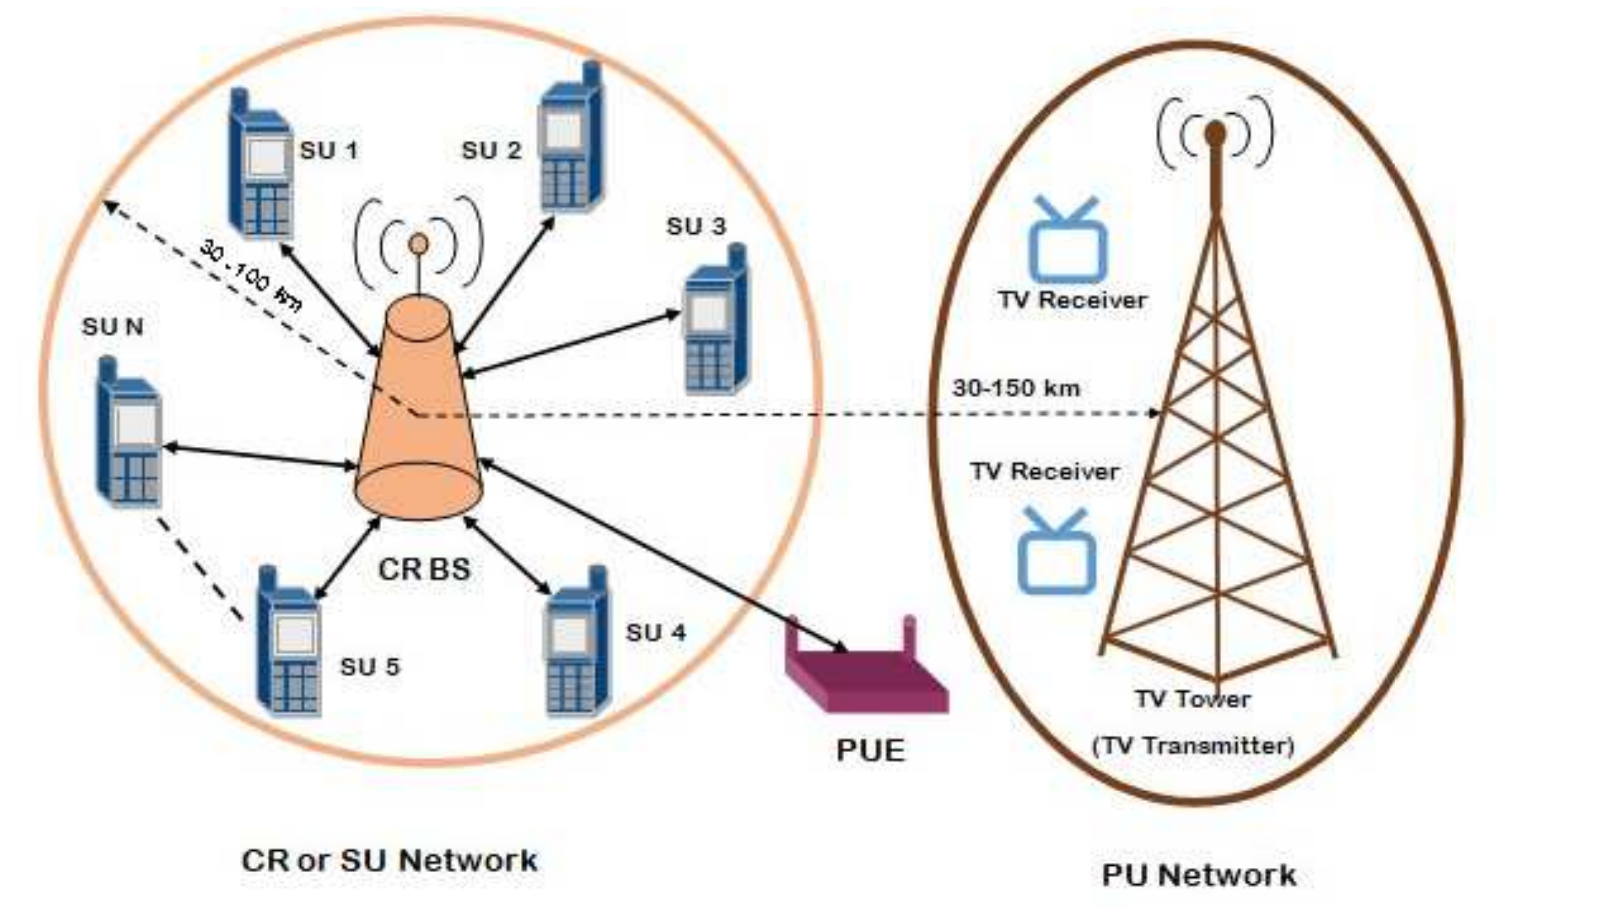
\includegraphics[width=0.9\linewidth]{Figures/chapter1/location-based PUEA detection.png}
    \caption{Location-based PUEA detection \cite{ref20}}
    \label{fig:enter-label}
\end{figure}

\subsection{Signal Characteristic-based Methods}
Several researchers have exploited unique signal characteristics to identify PUEA \cite{ref11,ref6}. For instance, \cite{ref11} utilized cyclostationarity features of signals, while employed cross-layer detection techniques combining PHY and MAC layer information \cite{ref5}. These approaches typically perform well in controlled environments but may struggle when attackers precisely mimic legitimate signal characteristics\cite{ref17}.

\subsection{Machine Learning-based Methods}
Recent years have witnessed growing interest in applying machine learning techniques for PUEA detection  \cite{ref9, ref23}. These approaches train classifiers using features extracted from signal measurements to distinguish between legitimate and malicious transmissions \cite{ref22,ref19}. While promising, many existing machine learning approaches have not been systematically evaluated across varying spatial scenarios and attacker presence levels \cite{ref13}.
 
\chapter{Literature Review}
\label{Chapter3}
\lhead{Chapter 3. \emph{Literature Review}}

% {\LARGE\textbf{Literature Review Table: \ref{tab:LR_view1}
% Table: \ref{tab:LR_view2}}}

\begin{table}[]
    \centering
\begin{tabular}{|p{0.5cm}|p{2.5cm}|p{1.0cm}|p{3.2cm}|p{2.9cm}|p{2.8cm}|}
\hline
\textbf{SL. No.} & \textbf{Author} & \textbf{Date} & \textbf{Title} & \textbf{Contribution} & \textbf{Methodology} \\

\hline
1 & Ian F. Akyildiz, Won-Yeol Lee, Mehmet C. Vuran *, Shantidev Mohan & 2 May 2006 & NeXt generation/dynamic spectrum access/cognitive
radio wireless networks: A survey & xG networks (cognitive radio-based) as a solution to inefficient spectrum usage and analyzes their architecture, key functions, and impact on network protocols & survey-based analysis is used to explore functionalities, challenges, and cross-layer issues in xG networks.\\
\hline
2 & Ruiliang Chen, Jung-Min Park, and Jeffrey H. Reed & 31 Jan, 2008 & Defense against Primary User Emulation Attacks in
Cognitive Radio Networks & Primary User Emulation (PUE) attack as a serious threat to spectrum sensing in cognitive radio networks and proposes a localization-based defense mechanism, LocDef, to detect such attacks & proposed LocDef scheme using non-interactive localization to verify transmitter identity \\
\hline
3 & Z. Jin, S. Anand and K.P. Subbalakshmi & 11 Aug, 2009 & Detecting Primary User Emulation Attacks in Dynamic Spectrum Access Networks & Proposed a non-location-based method to detect PUEA in cognitive radio networks & Used Fenton’s approximation and WSPRT, supported by simulations\\
\hline
4 & Zesheng Chen, Todor Cooklev, Chao Chen, and Carlos Pomalaza-R´aez & 02 Feb, 2010 & Modeling Primary User Emulation Attacks and
Defenses in Cognitive Radio Networks & advanced PUEA strategies and proposes an effective countermeasure using channel invariants & estimation and learning techniques for both attack and defense, demonstrating their impact through comparative analysis\\

\hline
5 & Yao Liu, Peng Ning and Huaiyu Dai & 08 Jul, 2010 & Authenticating Primary Users' Signals in Cognitive Radio Networks via Integrated Cryptographic and Wireless Link Signatures & primary user authentication method in cognitive radio networks using helper nodes that combine cryptographic and physical-layer link signatures to detect malicious signal emulation & Training-free physical layer authentication technique leveraging helper nodes placed near primary users, conforming to FCC constraints and evaluated through theoretical design \\
\hline
6 & Bilal Naqvi, Imran Rashid, Fasisal Riaz and Baber Aslam & 10 Feb, 2014 & Primary User Emulation attack and their mitigation strategies: A survey &  Primary User Emulation (PUE) attacks in cognitive radio networks, analyzes existing mitigation techniques, and highlights unaddressed gaps requiring future solutions & survey-based approach that critically examines current PUE attack defenses and identifies their limitations to motivate further research.\\

\hline

\end{tabular}
    \caption{Literature Review}
    \label{tab:LR_view1}
\end{table}

\begin{table}[]
    \centering
\begin{tabular}{|p{0.5cm}|p{2.5cm}|p{1.1cm}|p{2.8cm}|p{2.8cm}|p{2.8cm}|}
\hline
\textbf{SL. No.} & \textbf{Author} & \textbf{Date} & \textbf{Title} & \textbf{Contribution} & \textbf{Methodology} \\
\hline
7 & Mohammad Javad Saber and Seyed Mohammad Sajad Sadough & 05 Jan, 2015 & Robust cooperative spectrum sensing in cognitive radio networks under multiple smart primary user emulation attacks &  cooperative spectrum sensing scheme to counter multiple smart Primary User Emulation Attacks (PUEAs) in cognitive radio networks by optimizing signal fusion to improve detection accuracy & Simulation-based evaluation of a fusion-center-driven sensing approach that maximizes the Cognitive Signal-to-Interference-plus-Noise Ratio (CSINR) for robust detection under coordinated PUEAs \\
\hline
8 & Dinu Mary Alias, Ragesh G. K & 15 Sep, 2016 & Cognitive Radio Networks: A Survey & Dynamic spectrum access improves spectrum efficiency & Centralized sharing, Distributed sharing \\
\hline
9 & D. L. Chaitanya and K. M. Chari & 04 May 2017 & Defense against PUEA and SSDF attacks in cognitive radio networks & Evaluate the performance of CRN. Also to mitigate the effect of SSDF attack & Hard Decision fusion rules are applied such as AND, OR and K out of N rules \\
\hline
10 & Khaled Mohammed Saifuddin et al. & 01 Sep, 2017 & Detection of Primary User Emulation Attack in Cognitive Radio Environment & Different methods to model communication channels and improve signal measurement accuracy & Filter and cyclostationary feature detection, spectrum decision \\
\hline
11 & Ishu Gupta, O. P. Sahu & 01 Feb, 2018 & An Overview of Primary User Emulation Attack in Cognitive Radio Networks & General overview of cognitive radio security issues with focus on PUEA & Energy detection, cyclostationary feature based detection \\
\hline

12 & Khatereh Akbari, Jamshid Abouei & 01 May, 2018 & Signal Classification for Detecting Primary User Emulation Attack in Centralized CRNs & Effective sequential scheme to identify PUE attack in CRNs & Bayesian nonparametric clustering approach based on DPMM \\
\hline
13 & N. Sureka and K. Gunaseelan & 11 Mar 2019 & Detection \& Defense against Primary User Emulation Attack in Dynamic Cognitive Radio Networks & Minimum interference to primary transmissions & Yardstick based Threshold Allocation (YTA) \\
\hline
14 & S. Arun \& G. Umamaheswari & 29 Apr 2019 & An Adaptive Learning-Based Attack Detection Technique for Mitigating Primary User Emulation in Cognitive Radio Networks & Proposes adaptive learning-based attack detection for PUEA, Enhances signal classification and SU communication rate. & Adaptive learning-based attack detection method, Cyclostationary feature analysis for signal classification \\
\hline
\end{tabular}
    \caption{Literature Review}
    \label{tab:LR_view1}
\end{table}


\begin{table}[]
    \centering
\begin{tabular}{|p{0.5cm}|p{2.5cm}|p{1.1cm}|p{2.8cm}|p{2.8cm}|p{2.8cm}|}
\hline
\textbf{SL. No.} & \textbf{Author} & \textbf{Date} & \textbf{Title} & \textbf{Contribution} & \textbf{Methodology} \\
\hline
15 & Wangjam Niranjan Singh, Ningrinla Marchang
and Amar Taggu & 25 Sept, 2019 & Mitigating SSDF attack using distance-based outlier approach in cognitive radio networks & Diving into two groups, non-outlier set and candidate set
 & Distance-based outlier approach \\
 \hline
 16 & Nikita Mishra, Sumit Srivastava and Shivendra Nath Sharan & 16 Jun, 2020 & Countermeasures for Primary User Emulation Attack: A Comprehensive Review & Research on PUEA in cognitive radio networks, offering insights and future strategies for secure and energy-efficient CR systems & survey and synthesis of existing literature, concluding with recommendations for next-generation CR security \\
\hline
17 & Avila Jayapalan, Prem Savarinathan, Jagathi Chenna Reddy & 07 Feb 2021 & Detection and Defense of PUEA in Cognitive Radio Network & PUEA detection using feature detection-based sensing with thresholds, Game model for strategic defense decisions against attackers. & Feature detection-based sensing with double threshold for PUEA detection, Game model for strategic defense decisions against attackers. 
\\
\hline
18 & Bishal Chhetry, Ningrinla Marchanga & 21 Jun, 2021 & Detection Of PUEA In CRNs Using One-Class Classification & One-class classification used for detecting PUEA & Isolation Forest, Support Vector Machine, MCD and LOF \\
\hline
19 & Grace Olaeru, Henry Ohize, Abubakar Saddiq Mohammed and Umar Suleiman Dauda & 24 Mar, 2022 & Optimal Detection Technique for Primary User Emulator in Cognitive Radio Network & Detects PUEA in CRNs using TDOA-based localization enhanced with optimization algorithms, identifying MPSO as the most effective & Simulation-based comparison of PSO, NBA, and MPSO using MATLAB and Monte Carlo trials, evaluated via MSE and CDF \\
\hline
20 & Amar Taggu, Ningrinla Marchang & 05 Jul, 2022 & A Density-based Clustering Approach to detect Colluding SSDF Attackers & Proposed DBSCAN-based technique for detecting Colluding SSDF attacks & Density-Based Spatial Clustering (DBSCAN) \\

\hline
21 & H. Thakkar and S. Goswami & 09 Aug 2023 & The Cluster-based Cognitive Radio Sensor Networks that are Wireless Aware of PUEA and SSDF Attacks & Resolve Spectrum Sensing
Data Falsification attack and Primary User Emulation attack & regression based spectrum
sensing data falsification attack detection technique and
mathematical SHA with Digital Signature \\
\hline
22 & C. Ambhika & 01 Apr 2024 & Discrimination of primary user emulation attack on cognitive radio networks using machine learning based spectrum sensing scheme & Detection and prevention of primary user emulation attack.
Improved sensing ability and energy efficiency in networks. & Time-Distance with signal Strength Evaluation (TDSE),
Extreme Machine Learning (EML) algorithm \\
\hline
\end{tabular}
    \caption{Literature Review}
    \label{tab:LR_view2}
\end{table}



This section presents a comprehensive analysis of the existing literature on Primary User Emulation Attack (PUEA) detection and mitigation techniques in Cognitive Radio Networks. The review is organized into major categories based on the methodological approaches employed by researchers.


Energy detection remains one of the fundamental approaches for spectrum sensing and PUEA detection in cognitive radio networks. This technique relies on measuring the energy of received signals and comparing them against predefined thresholds to determine the presence or absence of primary users.

Gupta and Sahu \cite{ref1} provided a comprehensive overview of primary user emulation attacks, emphasizing the effectiveness of energy detection methods combined with cyclostationary feature-based detection. Their work titled ``An Overview of Primary User Emulation Attack in Cognitive Radio Networks" highlighted that energy detection, while simple to implement, suffers from limitations in low Signal-to-Noise Ratio (SNR) environments and requires careful threshold selection to minimize false alarm rates. The authors comprehensively analyzed various detection techniques and established the foundation for understanding PUEA vulnerabilities in cognitive radio systems.
Chen et al. \cite{ref4} developed defense mechanisms against primary user emulation attacks in cognitive radio networks, focusing on authentication-based approaches. Their work ``Defense against primary user emulation attacks in cognitive radio networks" established fundamental defense strategies that complement energy detection methods by providing cryptographic verification of legitimate primary user signals.
Jin et al. \cite{ref6} proposed detection methods for primary user emulation attacks in dynamic spectrum access networks. Their research ``Detecting primary user emulation attacks in dynamic spectrum access networks" introduced novel approaches for identifying emulated signals through statistical analysis of signal characteristics and temporal patterns, providing a foundation for threshold-based detection systems.


The application of machine learning techniques has emerged as a promising approach for addressing the complexities of PUEA detection. These methods leverage pattern recognition and statistical learning to identify subtle differences between legitimate primary user signals and emulated signals.
Wang et al. \cite{ref9} proposed machine learning techniques for primary user emulation attack detection in cognitive radio in their research ``Primary user emulation attack detection in cognitive radio using machine learning techniques". Their approach leverages advanced algorithms to analyze spectrum sensing data and identify patterns indicative of emulation attacks, demonstrating superior performance in dynamic environments where traditional methods may fail.
Chhetry and Marchang \cite{ref23} explored one-class classification methods for PUEA detection in their comprehensive study ``Detection of PUEA in CRNs using one-class classification", employing multiple algorithms including Isolation Forest, Support Vector Machine (SVM), Minimum Covariance Determinant (MCD), and Local Outlier Factor (LOF). Their comparative study revealed that one-class classification is particularly effective when labeled data for attacks is scarce, as it only requires examples of normal behavior for training. The Isolation Forest algorithm showed superior performance in detecting novel attack patterns due to its ability to isolate anomalies through random partitioning.
Arun and Umamaheswari \cite{ref19} developed an adaptive learning-based attack detection technique for mitigating primary user emulation in cognitive radio networks. Their work ``An Adaptive Learning-Based Attack Detection Technique for Mitigating Primary User Emulation in Cognitive Radio Networks" demonstrates how machine learning can adapt to evolving attack strategies, providing robust detection capabilities that improve over time through continuous learning.


Cooperative spectrum sensing leverages the spatial diversity of multiple secondary users to improve detection accuracy and mitigate the effects of shadowing and fading. This approach is particularly effective against sophisticated PUEA strategies that may fool individual sensors.
Huang et al. \cite{ref8} focused on robust collaborative spectrum sensing in the presence of primary user emulation attacks in their work ``Robust collaborative spectrum sensing in the presence of primary user emulation attacks". Their methodology develops advanced fusion techniques that can maintain detection accuracy even when some participating nodes are compromised by attackers. The collaborative approach enhances overall network resilience by leveraging the spatial diversity of multiple sensing nodes.
Singh et al. \cite{ref14} proposed a distance-based outlier approach for mitigating SSDF attacks in their paper ``Mitigating SSDF Attack using Distance-based Outlier approach in Cognitive Radio Networks", which complements PUEA detection efforts. Their method divides secondary users into two groups: a non-outlier set consisting of trusted users and a candidate set containing potentially malicious users. The distance-based clustering algorithm identifies outliers by measuring the statistical distance between user reports and the expected behavior patterns.
Thakkar and Goswami \cite{ref12} addressed the challenges of wireless cognitive radio sensor networks by developing cluster-based approaches that are aware of both PUEA and SSDF attacks in their research ``The Cluster-based Cognitive Radio Sensor Networks that are Wireless Aware of PUEA and SSDF Attacks". Their methodology combines regression-based spectrum sensing data falsification attack detection with mathematical Secure Hash Algorithm (SHA) and digital signatures for authentication. This multi-layered security approach ensures both detection accuracy and data integrity in distributed sensing scenarios.


Clustering algorithms have gained significant attention for PUEA detection due to their ability to group similar signal characteristics and identify anomalous behaviors that may indicate attacks.
Taggu and Marchang \cite{ref21} proposed a density-based clustering approach using DBSCAN (Density-Based Spatial Clustering) to detect colluding SSDF attackers in their research ``A Density-based Clustering Approach to detect Colluding SSDF Attackers in Cognitive Radio Networks". Their method is particularly effective against coordinated attacks where multiple malicious users collaborate to deceive the network. The DBSCAN algorithm identifies clusters of normal behavior and flags data points that fall outside these clusters as potential attacks. The density-based approach is robust against noise and can identify clusters of arbitrary shapes, making it suitable for complex attack scenarios.
Luo et al. \cite{ref13} developed a novel clustering-based feature extraction method for PUEA detection in their work ``A novel clustering-based feature extraction method for PUEA detection". Their approach combines clustering algorithms with feature extraction techniques to identify distinctive patterns in spectrum sensing data that can effectively distinguish between legitimate and emulated signals.
The clustering-based approaches demonstrate particular strength in scenarios where attackers employ sophisticated strategies to mimic legitimate user behavior. By analyzing the clustering patterns of sensing reports over time, these methods can identify subtle deviations that may not be apparent through individual signal analysis.



Feature-based detection methods focus on analyzing specific characteristics of received signals to distinguish between legitimate and emulated transmissions. These approaches exploit the inherent differences in signal properties that are difficult for attackers to replicate perfectly.
Jin et al. \cite{ref15} developed detection methods for primary user emulation attacks in dynamic spectrum access networks in their paper ``Detecting primary user emulation attacks dynamic spectrum access networks". Their approach focuses on analyzing signal characteristics and temporal patterns to identify emulated signals, providing a foundation for feature-based detection systems that can adapt to various attack strategies.
Lafia et al. \cite{ref11} proposed a signal processing-based model for primary user emulation attacks detection in cognitive radio networks in their work ``Signal Processing-based Model for Primary User Emulation Attacks Detection in Cognitive Radio Networks". Their approach combines advanced signal processing techniques with feature extraction methods to create robust detection mechanisms that can identify subtle differences between legitimate and emulated signals.
The feature-based detection approaches often combine multiple signal characteristics such as power spectral density, modulation parameters, and temporal patterns to create comprehensive feature vectors that can effectively distinguish between legitimate and emulated signals. These methods demonstrate particular effectiveness in scenarios where attackers attempt to closely mimic legitimate primary user characteristics.



Authentication-based approaches represent a fundamental class of defense mechanisms against PUEA, focusing on verifying the legitimacy of primary user signals through cryptographic and signal-based authentication methods.
Liu et al. \cite{ref5} developed an integrated approach for ``Authenticating primary users' signals in cognitive radio networks via integrated cryptographic and wireless link signatures". Their method combines cryptographic techniques with wireless link characteristics to create a robust authentication framework that can verify the legitimacy of primary user transmissions, making it extremely difficult for attackers to successfully emulate authenticated signals.
Chen et al. \cite{ref17} presented analytical models for primary user emulation attacks and defenses in their work ``Modeling primary user emulation attacks and defenses in cognitive radio networks". Their research provides theoretical foundations for understanding the interaction between attackers and defense mechanisms, offering insights into optimal authentication strategies and their effectiveness against various attack scenarios.
Anand et al. \cite{ref16} developed ``An Analytical Model for Primary User Emulation Attacks in Cognitive Radio Networks" that provides mathematical frameworks for understanding attack strategies and defense mechanisms. Their analytical approach helps in designing more effective authentication protocols by predicting attacker behavior and system vulnerabilities.



Several foundational works have established the theoretical framework for understanding cognitive radio networks and PUEA threats, providing comprehensive surveys and establishing research directions.

Alias and Ragesh \cite{ref2} provided a comprehensive survey titled ``Cognitive Radio networks: A survey" that established the fundamental principles of cognitive radio networks. Their work demonstrated how dynamic spectrum access can be implemented through various architectural approaches, laying the groundwork for understanding both the opportunities and vulnerabilities in cognitive radio systems.
Akyildiz et al. \cite{ref3} presented a foundational survey on ``Next generation/dynamic spectrum access/cognitive radio wireless networks: A survey" that established the theoretical framework for cognitive radio technology. Their comprehensive analysis covers the evolution from traditional spectrum management to dynamic spectrum access, providing the conceptual foundation that underlies much of the subsequent research on security vulnerabilities including PUEA.
Naqvi et al. \cite{ref7} provided a comprehensive review of ``Primary User Emulation attack and their mitigation strategies: A survey" that systematically analyzed various PUEA attack vectors and corresponding defense mechanisms. Their survey established a taxonomy of attack types and mitigation approaches, serving as a critical reference for researchers developing new detection and defense strategies.
Parvin et al. \cite{ref25} conducted an extensive survey on ``Cognitive radio network security: A survey" that provides a broad perspective on security challenges in cognitive radio networks, including PUEA as well as other security threats. Their work establishes the broader security context within which PUEA detection and mitigation techniques operate.


Recent advances in deep learning have opened new possibilities for PUEA detection, offering sophisticated pattern recognition capabilities that can adapt to evolving attack strategies.
Zhao \cite{ref22} developed ``A reliable spectrum sensing method based on deep learning for primary user emulation attack detection in cognitive radio network". Their approach leverages deep neural networks to analyze complex patterns in spectrum sensing data, demonstrating superior performance in detecting sophisticated emulation attacks that may fool traditional detection methods. The deep learning model can automatically extract relevant features and adapt to new attack patterns through continuous learning.
Olaleru et al. \cite{ref20} proposed an ``Optimal Detection Technique for Primary User Emulator in Cognitive Radio Network" that incorporates advanced optimization techniques for improving detection accuracy. Their work focuses on developing optimal detection strategies that can maximize detection probability while minimizing false alarm rates.
Mishra et al. \cite{ref24} provided a comprehensive review of ``Countermeasures for primary user emulation attack: A comprehensive review" that systematically analyzes various defense mechanisms including emerging deep learning approaches. Their survey highlights the evolution from traditional signal processing methods to advanced machine learning and deep learning techniques for PUEA detection.



Despite the significant progress in PUEA detection techniques, several critical limitations persist across the reviewed literature that hinder the development of comprehensive and robust detection systems. Most studies concentrate on a single detection algorithm without comprehensive comparative analysis across different methodological approaches under varying conditions, as evidenced in the works of Gupta and Sahu \cite{ref1}, Jin et al. \cite{ref6}, and Chhetry and Marchang \cite{ref23}, which focus exclusively on their respective detection methods without systematic comparison with alternative approaches. There is insufficient exploration of how different algorithms perform across varying spatial configurations and attacker distributions, with studies like Chen et al. \cite{ref4} and Arun and Umamaheswari \cite{ref19} primarily evaluating their methods under limited spatial scenarios. Few studies systematically combine multiple detection techniques to leverage the strengths of different approaches, with notable exceptions being the works of Liu et al. \cite{ref5} and Thakkar and Goswami \cite{ref12}, though even these hybrid approaches remain limited in scope. Many proposed methods lack rigorous statistical validation of performance improvements, particularly in terms of statistical significance testing, as observed in the machine learning approaches by Wang et al. \cite{ref9} and the clustering methods by Taggu and Marchang \cite{ref21}, which rely primarily on simulation results without comprehensive statistical analysis. Additionally, most research focuses on simulation-based validation with limited consideration of practical implementation challenges and real-world constraints, as highlighted in the survey by Naqvi et al. \cite{ref7} and the comprehensive review by Mishra et al. \cite{ref24}, indicating a significant gap between theoretical proposals and practical deployment considerations. These gaps highlight the need for more comprehensive comparative studies and the development of robust hybrid detection mechanisms that can effectively address the evolving nature of PUEA threats in modern cognitive radio networks.



\section{\textbf{Countermeasure}}
Primary User Emulation Attacks (PUEA) pose significant threats to Cognitive Radio Networks (CRNs) by misleading secondary users about the availability of spectrum, necessitating the development of comprehensive countermeasures and mitigation strategies to ensure robust network security \cite{ref1,ref4,ref24}. The most effective approaches include cooperative spectrum sensing, which involves multiple secondary users collaboratively sensing the spectrum and sharing their observations to better distinguish between legitimate primary user signals and emulated signals, thereby enhancing detection accuracy and reducing false positives through collective sensing capabilities \cite{ref8}. Energy detection and thresholding methods measure the energy of received signals and compare them to predefined thresholds, adjusting detection parameters based on environmental conditions and historical data to minimize false alarms while maintaining effectiveness in low-noise environments. Feature-based detection techniques analyze specific signal characteristics such as modulation type and signal shape, comparing these features against known profiles of legitimate primary user signals to identify anomalies indicative of PUEA attacks \cite{ref11}. Location verification methods add an additional security layer by verifying the geographical location of signal sources using GPS data or other location-based technologies to ensure signals originate from expected locations where legitimate primary users operate. Advanced machine learning techniques utilize algorithms such as Support Vector Machines (SVM) and neural networks to detect PUEA by analyzing patterns in spectrum sensing data, offering the capability to adapt to new attack patterns and improve detection rates over time through continuous learning \cite{ref9,ref19,ref23}. Adaptive resource allocation strategies dynamically adjust power levels and communication parameters based on current network conditions and potential attack presence, enhancing overall network efficiency while reducing the likelihood of successful attacks \cite{ref3}. Cross-layer approaches integrate information from multiple network stack layers (physical, MAC, network) to provide a holistic view of network conditions and improve detection capabilities through data correlation from different layers. Trust-based mechanisms establish frameworks among secondary users to assess the reliability of their reports, giving more weight to users with accurate reporting histories while monitoring or excluding those suspected of malicious behavior, thereby encouraging cooperation and helping identify potential attackers \cite{ref5,ref8}. Mitigating Primary User Emulation Attacks in Cognitive Radio Networks requires this multifaceted approach that combines various detection and defense strategies, and by employing cooperative sensing, advanced detection techniques, and adaptive resource management, CRNs can enhance their resilience against PUEA and ensure efficient spectrum utilization, while ongoing research continues to explore innovative methods to further strengthen these defenses and improve the overall security of cognitive radio networks \cite{ref3,ref8,ref24,ref25}.
\chapter{Methodology}
\label{C\begin{table}[h]
\centering
\\begin{table}[h]
\centering
\caption{Distance Scenario Configurations}
\label{tab:scenarios}
\begin{tabular}{|l|l|l|}
\hline
\textbf{Scenario} & \textbf{PU-PUEA Distance} & \textbf{Detection Challenges} \\
\hline
A (Far) & 100 units & Signal attenuation effects \\
B (Medium) & 65 units & Moderate power requirements \\
C (Close) & 30 units & High signal similarity \\
\hline
\end{tabular}
\end{table} Configuration Parameters}
\label{tab:system_config}
\begin{tabular}{|l|l|}
\hline
\textbf{Parameter} & \textbf{Value} \\
\hline
Network Topologies & 75 \\
Secondary Users per Topology & 30  \\
Geographical Area & 150×150 units \\
Time Slots per Scenario & 400  \\
\hline
\end{tabular}
\end{table}d{Chapter 4. \emph{Methodology}} 

This chapter presents the comprehensive methodology for Primary User Emulation Attack (PUEA) detection in Cognitive Radio Networks, implementing an integrated multi-topology evaluation framework with advanced machine learning clustering techniques and distance-based classification enhancement algorithms. The methodology encompasses experimental framework design, network topology generation, signal propagation modeling, statistical feature extraction, enhanced clustering algorithms, classification refinement techniques, and performance evaluation protocols. The systematic approach evaluates detection performance across 75 distinct network topologies establish robust statistical foundations for PUEA detection capability assessment.

The experimental framework establishes a comprehensive evaluation structure designed to assess Primary User Emulation Attack detection performance across diverse network configurations and attack scenarios. The integrated multi-topology PUEA detection system implements a hierarchical evaluation approach that systematically varies network parameters, spatial configurations, attack penetration levels, clustering methods, and classification techniques to provide thorough performance characterization.

The experimental design implements a hierarchical structure of five levels as shown in Table \ref{tab:hierarchy} that allows systematic evaluation in multiple dimensions of the network configuration and algorithmic parameters. This hierarchical approach ensures comprehensive coverage of realistic deployment scenarios while maintaining statistical rigor and computational feasibility.
 
\begin{table}[h]
\centering
\caption{Hierarchical Evaluation Structure Parameters}
\label{tab:hierarchy}
\begin{tabular}{|l|l|l|}
\hline
\textbf{Level} & \textbf{Parameter} & \textbf{Values/Range} \\
\hline
Level 1 & Network Topologies & 75 distinct configurations \\
Level 2 & Distance Scenarios & A (100 units), B (65 units), C (30 units) \\
Level 3 & PUEA Penetration & 10\%, 20\%, 30\%, 40\%, 50\% \\
Level 4 & Clustering Methods & K-means, Spectral, Agglomerative \\
Level 5 & Classification Enhancement & Original, KNN (R=5), Means-based \\
\hline
\textbf{Total Combinations} & \multicolumn{2}{|l|}{3,375 unique parameter sets} \\
\hline
\end{tabular}
\end{table}

The system configuration establishes standardized parameters that ensure consistent experimental conditions while enabling meaningful comparative analysis across different algorithmic approaches as shown in Table \ref{tab:system_config}

\begin{table}[h]
\centering
\caption{System Configuration Parameters}
\label{tab:system_config}
\begin{tabular}{|l|l|l|}
\hline
\textbf{Parameter} & \textbf{Value} \\
\hline
Network Topologies & 75 \\
Secondary Users per Topology & 30  \\
Geographical Area & 150×150 units \\
Time Slots per Scenario & 400  \\
\hline
\end{tabular}
\end{table}

Three distinct distance scenarios are implemented to represent different geographical attack configurations commonly encountered in cognitive radio deployments. Each scenario reflects specific operational characteristics and spatial relationships between primary users, adversarial entities, and secondary user networks as shown in Table \ref{tab:scenarios}

\begin{table}[h]
\centering
\caption{Distance Scenario Configurations}
\label{tab:scenarios}
\begin{tabular}{|l|l|l|l|}
\hline
\textbf{Scenario} & \textbf{PU-PUEA Distance} & \textbf{Detection Challenges} \\
\hline
A (Far) & 100 units & Signal attenuation effects \\
B (Medium) & 65 units & Moderate power requirements \\
C (Close) & 30 units & High signal similarity \\
\hline
\end{tabular}
\end{table}

The topology generation algorithm creates diverse network configurations through systematic parameter variation while ensuring reproducible results through controlled random number generation. The mathematical framework enables precise positioning of network entities within the standardized geographical area while maintaining realistic spatial relationships.

The signal propagation model implements a comprehensive framework that accurately represents wireless channel characteristics in cognitive radio environments. The model incorporates both deterministic path loss components and stochastic shadowing effects to provide realistic signal propagation modeling across diverse environmental conditions and spatial configurations.

The received power calculation follows an enhanced path loss equation that combines distance-dependent attenuation with stochastic channel variations:

\begin{equation}
P_r = P_t r^{-\alpha} e^{a\beta}
\end{equation}

where:
\begin{itemize}
\item $P_t$: Transmit power in linear scale
\item $P_r$: Received power in linear scale
\item $r$: Distance between transmitter and receiver in units
\item $\alpha$: Path loss exponent reflecting environmental characteristics
\item $a$: Scaling factor for stochastic effects
\item $\beta$: Random variable representing shadowing and fading effects
\end{itemize}

The power law distance dependence with exponential stochastic component accurately models signal attenuation in wireless environments while the multiplicative exponential term accounts for environmental variations and multi-path propagation effects commonly observed in cognitive radio deployments.

The channel model incorporates realistic parameter distributions based on empirical wireless propagation studies and cognitive radio deployment scenarios. Each parameter follows carefully selected probability distributions that reflect observed variations in realistic operating environments as shown in Table \ref{tab:channel_params}

\begin{table}[h]
\centering
\caption{Channel Model Parameters}
\label{tab:channel_params}
\begin{tabular}{|l|l|l|l|}
\hline
\textbf{Parameter} & \textbf{Distribution} & \textbf{Range} & \textbf{Physical Interpretation} \\
\hline
Path Loss Exponent ($\alpha$) & Uniform & [2, 6] & Free space to dense urban \\
Shadowing ($S$) & Uniform & [4, 12] dB & Environmental variations \\
PU Transmit Power & Constant & 15 dB & Baseline reference signal \\
PUEA Transmit Power & Uniform & [25, 35] dB & High-power attack signals \\
\hline
\end{tabular}
\end{table}

The time slot-based simulation incorporates 400 time slots per scenario to enable modeling of temporal channel variations while maintaining statistical consistency for performance evaluation. Each time slot represents an independent channel realization with randomly generated path loss exponent, shadowing values, and PUEA transmit power according to the specified distributions.

The feature extraction process transforms received power measurements into statistical descriptors that characterize signal propagation patterns and enable effective clustering analysis for PUEA detection. The comprehensive approach extracts five statistical features from received power measurements across 30 secondary user locations, providing sufficient dimensionality for meaningful clustering while maintaining computational efficiency.

The statistical feature extraction framework implements mathematically rigorous descriptors that capture different aspects of received power distributions across secondary user networks. Each feature provides unique information about signal propagation characteristics that distinguish between legitimate primary user transmissions and adversarial PUEA signals as shown in Table \ref{tab:features}.

\begin{table}[h]
\centering
\caption{Statistical Features and Their Properties}
\label{tab:features}
\begin{tabular}{|l|l|l|l|}
\hline
\textbf{Feature} & \textbf{Mathematical Form} \\
\hline
$F_1$ (Mean) & $\frac{1}{N}\sum P_i$  \\
$F_2$ (Variance) & $\frac{1}{N}\sum (P_i - F_1)^2$  \\
$F_3$ (Median) & 50th percentile \\
$F_4$ (Q1) & 25th percentile  \\
$F_5$ (Q3) & 75th percentile \\
\hline
\end{tabular}
\end{table}

The dataset construction process implements systematic procedures for creating training and evaluation datasets with different PUEA penetration levels (10\%, 20\%, 30\%, 40\%, 50\%). Each penetration level represents the proportion of time slots containing PUEA transmissions relative to legitimate primary user transmissions, enabling assessment of detection performance under varying attack intensity conditions as shown in Table \ref{tab:penetration}

\begin{table}[h]
\centering
\caption{PUEA Penetration Level Configuration}
\label{tab:penetration}
\begin{tabular}{|l|l|l|l|}
\hline
\textbf{Penetration Level} & \textbf{PUEA Samples} & \textbf{PU Samples} & \textbf{Total Samples} \\
\hline
10\% & 40 & 360 & 400 \\
20\% & 80 & 320 & 400 \\
30\% & 120 & 280 & 400 \\
40\% & 160 & 240 & 400 \\
50\% & 200 & 200 & 400 \\
\hline
\end{tabular}
\end{table}

The Manhattan distance matrix calculation implements the $L_1$ norm across the five-dimensional statistical feature space:

\begin{equation}
d_{Manhattan}(x_i, x_j) = \sum_{k=1}^{5} |x_{i,k} - x_{j,k}|
\end{equation}

where $x_{i,k}$ represents the $k$-th feature of sample $i$ across the five extracted statistical features (mean, variance, median, Q1, Q3).

The selection of Manhattan distance over Euclidean alternatives is based on empirical performance analysis and theoretical considerations relevant to statistical feature clustering. Manhattan distance demonstrates superior robustness to outliers in the five-dimensional feature space while providing computational efficiency with O(n²) complexity scaling for distance matrix construction.

\section{Proposed Clustering Method for PUEA Detection}

The enhanced clustering framework implements three advanced algorithms with systematic parameter optimization and validation strategies to improve PUEA detection performance beyond baseline implementations. Each algorithm incorporates specific enhancements designed to address challenges in wireless signal classification and improve robustness to parameter variations.

The enhanced K-means clustering algorithm incorporates multiple improvements over standard implementations, including feature standardization, multiple random initializations, and inertia-based model selection for robust cluster identification.

\textbf{Feature Standardization Implementation:}
Feature standardization employs StandardScaler with zero mean and unit variance normalization to ensure equal feature contribution to distance calculations:

\begin{equation}
X_{standardized} = \frac{X - \mu_X}{\sigma_X}
\end{equation}

where $\mu_X$ and $\sigma_X$ represent feature-wise means and standard deviations across all samples.

\begin{algorithm}
\caption{Enhanced K-means Implementation}
\begin{algorithmic}[1]
\REQUIRE Features matrix $X$, number of clusters $k=2$
\STATE $scaler \leftarrow StandardScaler()$
\STATE $X_{scaled} \leftarrow scaler.fit\_transform(X)$
\STATE $best\_inertia \leftarrow \infty$
\STATE $best\_labels \leftarrow None$
\FOR{$seed$ in $range(5)$}
    \STATE $kmeans \leftarrow KMeans(n\_clusters=2, random\_state=seed, n\_init=10)$
    \STATE $labels \leftarrow kmeans.fit\_predict(X_{scaled})$
    \IF{$len(unique(labels)) = 2$ AND $kmeans.inertia < best\_inertia$}
        \STATE $best\_inertia \leftarrow kmeans.inertia$
        \STATE $best\_labels \leftarrow labels$
    \ENDIF
\ENDFOR
\RETURN $best\_labels$
\end{algorithmic}
\end{algorithm}


The enhanced spectral clustering algorithm implements data-driven parameter optimization through multiple sigma calculation strategies and balanced cluster validation to improve performance across diverse feature distributions as shown in Algorithm~\ref{alg:spectral_clustering}.


\begin{algorithm}
\caption{Spectral Clustering}
\label{alg:spectral_clustering}
\begin{algorithmic}[1]
\REQUIRE Feature vectors $\{F_1, F_2, \ldots, F_m\}$, number of clusters $K$
\ENSURE Cluster assignments $\{c_1, c_2, \ldots, c_m\}$
\STATE Compute the similarity matrix $S$ where $S_{ij}$ measures similarity between $F_i$ and $F_j$
\STATE Construct the degree matrix $D$ where $D_{ii} = \sum_{j} S_{ij}$
\STATE Compute the unnormalized Laplacian matrix $L = D - S$
\STATE Compute the first $K$ eigenvectors of $L$ to form matrix $U \in \mathbb{R}^{m \times K}$
\STATE Normalize each row of $U$ to have unit length (optional, for normalized spectral clustering)
\STATE Apply K-means clustering to the rows of $U$ to obtain cluster assignments
\STATE \RETURN Cluster assignments $\{c_1, c_2, \ldots, c_m\}$
\end{algorithmic}
\end{algorithm}

The enhanced agglomerative clustering algorithm implements linkage preference optimization with balance threshold enforcement and robust fallback strategies for improved clustering reliability across diverse distance matrix characteristics as shown in Algorithm~\ref{alg:En_Agglo_cluster_algo}.


\begin{algorithm}
\caption{Enhanced Agglomerative Clustering}
\label{alg:En_Agglo_cluster_algo}
\begin{algorithmic}[1]
\REQUIRE Distance matrix $D$
\STATE $best\_balance \leftarrow 0$
\STATE $best\_labels \leftarrow None$
\STATE $linkage\_methods \leftarrow [average, complete, single]$
\STATE $linkage\_bonus \leftarrow \{average: 0.2, complete: 0.1, single: 0.0\}$
\FOR{$linkage$ in $linkage\_methods$}
    \STATE $agg \leftarrow AgglomerativeClustering(n\_clusters=2, linkage=linkage, metric=precomputed)$
    \STATE $labels \leftarrow agg.fit\_predict(D)$
    \STATE $counts \leftarrow count\_unique(labels)$
    \STATE $balance \leftarrow \min(counts) / \max(counts)$
    \STATE $score \leftarrow balance + linkage\_bonus[linkage]$
    \IF{$balance \geq 0.15$ AND $score > best\_balance$}
        \STATE $best\_balance \leftarrow score$
        \STATE $best\_labels \leftarrow labels.copy()$
    \ENDIF
\ENDFOR
\RETURN $best\_labels$
\end{algorithmic}
\end{algorithm}


\section{Proposed Enhanced Clustering Method for PUEA
Detection}

The classification enhancement framework implements two sophisticated algorithms designed to refine clustering results and improve PUEA detection accuracy through distance-based classification techniques. These algorithms address limitations of standard clustering approaches by incorporating neighborhood analysis and distance-based refinement strategies.


The cluster identification process employs a size-based heuristic for distinguishing between PU and PUEA clusters based on realistic attack scenario assumptions. This approach leverages the typical operational characteristic that primary user samples outnumber PUEA samples in most cognitive radio deployment scenariosas shown in Algorithm~\ref{alg:Cluster_identifi}.

\textbf{Size-based Cluster Assignment:}
\begin{algorithm}
\caption{Cluster Identification}
\label{alg:Cluster_identifi}
\begin{algorithmic}[1]
\REQUIRE Cluster labels $L$, unique clusters $\{C_0, C_1\}$
\STATE $count_0 \leftarrow \sum(L = C_0)$
\STATE $count_1 \leftarrow \sum(L = C_1)$
\IF{$count_0 > count_1$}
    \STATE $PU\_cluster \leftarrow C_0$, $PUEA\_cluster \leftarrow C_1$
\ELSE
    \STATE $PU\_cluster \leftarrow C_1$, $PUEA\_cluster \leftarrow C_0$
\ENDIF
\RETURN $PU\_cluster$, $PUEA\_cluster$
\end{algorithmic}
\end{algorithm}

This heuristic is justified based on the assumption that PUEA penetration levels (10-50\%) result in minority cluster assignment to PUEA samples, making the larger cluster likely to represent legitimate primary user transmissions.

The KNN-based enhancement algorithm implements neighborhood analysis using R=5 nearest neighbors to refine clustering decisions through local density analysis. This approach identifies potential misclassifications by examining the neighborhood composition around each candidate point as shown in Algorithm~\ref{alg:knn_en_algo}.

\textbf{Neighbor Identification Process:}
For each candidate point $i$ in the candidate set, the algorithm identifies 5 nearest neighbors based on Manhattan distance matrix ordering:

\begin{equation}
N_R(i) = \{j : j \text{ among } R \text{ nearest neighbors of } i \text{ based on } d_{ij}\}
\end{equation}

\textbf{Classification Decision Framework:}
The classification decision counts neighbors in candidate set (cCand) versus normal set (cNormal) with PUEA classification when cCand > cNormal:

\begin{algorithm}
\caption{KNN Enhancement Algorithm}
\label{alg:knn_en_algo}
\begin{algorithmic}[1]
\REQUIRE Distance matrix $D$, candidate set $CandSet$, R=5
\STATE $outliers \leftarrow []$
\FOR{$i$ in $CandSet$}
    \STATE $distances\_with\_indices \leftarrow [(D[i][j], j)$ for $j \neq i]$
    \STATE Sort $distances\_with\_indices$ by distance
    \STATE $cCand \leftarrow 0$, $cNormal \leftarrow 0$
    \FOR{$j$ in first $\min(R, |distances\_with\_indices|)$ entries}
        \STATE $neighbor\_idx \leftarrow distances\_with\_indices[j][1]$
        \IF{$neighbor\_idx$ in $CandSet$}
            \STATE $cCand \leftarrow cCand + 1$
        \ELSE
            \STATE $cNormal \leftarrow cNormal + 1$
        \ENDIF
    \ENDFOR
    \IF{$cCand > cNormal$}
        \STATE $outliers.append(i)$
    \ENDIF
\ENDFOR
\RETURN $outliers$
\end{algorithmic}
\end{algorithm}

The means-based enhancement algorithm implements distance-based refinement through iterative evaluation of point assignments based on distance sum minimization as shown in Algorithm ~\ref{alg:means_enhancement}. This approach refines cluster assignments by comparing individual point distances to cluster centroids.

\textbf{Distance Sum Calculation:}
The algorithm computes total distance sums for candidate and normal sets:

\begin{align}
CandDist[i] &= \sum_{j=1}^{n} d_{ij} \text{ for } i \in CandSet \\
TotalCandDist &= \sum_{i \in CandSet} CandDist[i]
\end{align}

\textbf{Iterative Refinement Process:}
Point-by-point evaluation based on distance difference minimization:

\begin{algorithm}
\caption{Means-based Enhancement Algorithm}
\label{alg:means_enhancement}
\begin{algorithmic}[1]
\REQUIRE Distance matrix $D$, candidate set $CandSet$
\STATE Compute $CandDist$ and $NormDist$ for all points
\STATE $refined\_CandSet \leftarrow CandSet.copy()$
\STATE $refined\_NormalSet \leftarrow NormalSet.copy()$
\REPEAT
    \STATE $changes \leftarrow 0$
    \FOR{$i$ in $refined\_CandSet$}
        \STATE $CandDistMeans \leftarrow current\_TotalCandDist / |refined\_CandSet|$
        \STATE $NormDistMeans \leftarrow current\_TotalNormDist / |refined\_NormalSet|$
        \STATE $cand\_diff \leftarrow |CandDistMeans - CandDist[i]|$
        \STATE $norm\_diff \leftarrow |NormDistMeans - NormDist[i]|$
        \IF{$cand\_diff > norm\_diff$}
            \STATE Move $i$ from candidate to normal set
            \STATE $changes \leftarrow changes + 1$
        \ENDIF
    \ENDFOR
\UNTIL{$changes = 0$}
\RETURN $refined\_CandSet$
\end{algorithmic}
\end{algorithm}


The performance evaluation framework implements comprehensive metrics calculation and statistical analysis procedures to assess PUEA detection effectiveness across all experimental conditions. The framework incorporates detection rate and false detection rate calculations with robust statistical validation procedures.


The performance evaluation employs two primary metrics that characterize detection system effectiveness from complementary perspectives:

\textbf{Detection Rate (DR):} Proportion of correctly identified PUEA samples representing system sensitivity:

\begin{equation}
DR = \frac{\text{Correctly detected PUEA}}{\text{Total No. of PU}}
\end{equation}

\textbf{False Detection Rate (FDR):} Proportion of PU samples incorrectly classified as PUEA representing system specificity:

\begin{equation}
FDR = \frac{\text{No. of PU falsely detected as PUEA}}{\text{Total No. of PU}} 
\end{equation}

The complete evaluation pipeline processes unique parameter combinations, generating comprehensive performance characterization across all experimental dimensions as shown in \ref{tab:eval_pipeline}

The evaluation framework implements intermediate result saving mechanisms every 10 topologies to ensure progress preservation and enable memory management during extended computational experiments. This approach prevents data loss while providing checkpoint capabilities for experiment monitoring and debugging.

\begin{table}[h]
\centering
\caption{Evaluation Pipeline Computational Requirements}
\label{tab:eval_pipeline}
\begin{tabular}{|l|l|l|}
\hline
\textbf{Component} & \textbf{Quantity} & \textbf{Total Operations} \\
\hline
Network Topologies & 75 & Base configurations \\
Distance Scenarios & 3 per topology & 225 scenario evaluations \\
Penetration Levels & 5 per scenario & 1,125 penetration cases \\
Clustering Methods & 3 per case & 3,375 clustering operations \\
Enhancement Methods & 3 per clustering & 10,125 enhancement operations \\
Performance Measurements & 1 per enhancement & 10,125 measurements \\
\hline
\textbf{Total Unique Combinations} & \multicolumn{2}{|l|}{3,375 parameter sets} \\
\hline
\end{tabular}
\end{table}

The statistical validation framework ensures data integrity and experimental reproducibility through comprehensive validation and quality assurance protocols. To ensure reliable results, the framework implements multiple layers of data integrity checking, starting with feature value range validation, which confirms that mean values are within a $[-50, 50]~\text{dB}$ range, variance is non-negative with an upper bound of $100~\text{dB}^2$, percentile ordering is consistent ($Q_1 \le \text{Median} \le Q_3$), and statistical feature correlations are checked to detect errors. The framework also performs distance matrix validation to ensure symmetry ($d_{ij} = d_{ji}$), non-negativity ($d_{ij} \ge 0$), and a zero diagonal ($d_{ii} = 0$), alongside spot-checking the triangle inequality. Finally, clustering validation confirms the generation of exactly two clusters for binary classification, checks for cluster balance to prevent degenerate solutions, validates the convergence of iterative algorithms, and ensures label consistency across enhancement algorithms.

 
\chapter{Results \& Discussion}
\label{Chapter5}
\lhead{Chapter 5. \emph{Results \& Discussion}} 

\section{Results}

The comprehensive evaluation of Primary User Emulation Attack detection algorithms across three distance scenarios and five PUEA penetration levels (10\%, 20\%, 30\%, 40\%, 50\%) reveals significant performance variations among clustering approaches and spatial configurations, as detailed in Tables \ref{tab:scenario_performance} and \ref{tab:method_performance}. Table \ref{tab:scenario_performance} demonstrates clear distance-dependent performance patterns: Scenario A (Far Distance - 100 units) achieved average detection rates of 85.43\% with 8.49\% false detection rate, Scenario B (Medium Distance - 65 units) achieved 91.09\% detection rate with 6.34\% false detection rate, and Scenario C (Close Distance - 30 units) achieved the highest performance with 91.54\% detection rate and lowest 5.92\% false detection rate. Table \ref{tab:method_performance} provides comprehensive analysis of all method combinations, showing that K-means clustering methods demonstrate superior and consistent performance across all experimental conditions, with K-means Original achieving overall average detection rate of 91.36\% and false detection rate of 6.92\%, K-means KNN achieving 91.54\% detection rate with 6.84\% false detection rate, and K-means Means achieving 91.48\% detection rate with 6.83\% false detection rate. As shown in Table \ref{tab:method_performance}, the K-means Original method shows exceptional performance consistency, maintaining detection rates above 86\% even at 40\% PUEA penetration (86.67\%) and achieving peak performance of 96.67\% at 30\% PUEA penetration. Enhanced Spectral clustering methods show moderate performance with Enhanced Spectral KNN achieving the best spectral performance of 66.02\% average detection rate with 25.71\% false detection rate, while Enhanced Spectral Original achieved 61.60\% detection rate with 27.89\% false detection rate. Enhanced Agglomerative clustering exhibits consistent but lower performance, with Enhanced Agglomerative KNN achieving 62.69\% detection rate and 22.01\% false detection rate, outperforming both Enhanced Agglomerative Original (58.27\% detection rate, 24.19\% false detection rate) and Enhanced Agglomerative Means (61.83\% detection rate, 21.76\% false detection rate), as comprehensively detailed in Table \ref{tab:method_performance}.

\section{Discussion}

The experimental results presented in Tables \ref{tab:scenario_performance} and \ref{tab:method_performance} validate the fundamental hypothesis that spatial geometric configuration significantly impacts PUEA detection performance, with closer proximity scenarios consistently outperforming larger separation distances across all clustering algorithms. The progressive improvement shown in Table \ref{tab:scenario_performance} from Scenario A (85.43\% average detection rate) through Scenario B (91.09\%) to Scenario C (91.54\%) demonstrates a clear 6.11 percentage point improvement between far and close distance configurations, while false detection rates decrease correspondingly from 8.49\% to 5.92\%. Table \ref{tab:method_performance} clearly establishes K-means clustering as the dominant detection methodology, with all three K-means variants (Original, KNN, Means) achieving over 91\% average detection rates and maintaining false detection rates below 7\%, significantly outperforming both Enhanced Spectral and Enhanced Agglomerative approaches. The performance degradation patterns across PUEA penetration levels revealed in Table \ref{tab:method_performance} show critical deployment thresholds: K-means methods maintain detection rates above 86\% until 40\% penetration but show significant degradation at 50\% penetration (dropping to approximately 74\%), indicating practical operational limits for high-security applications. Enhanced clustering methods demonstrate substantial but limited improvement over baseline approaches, with Enhanced Spectral KNN showing 66.02\% average performance compared to Enhanced Spectral Original's 61.60\%, representing meaningful but insufficient advancement for critical security applications. The consistent performance ranking evident in Table \ref{tab:method_performance} (K-means variants $>$ Enhanced Spectral variants $>$ Enhanced Agglomerative variants) across all experimental conditions indicates robust algorithmic superiority that transcends specific deployment scenarios. Distance-dependent performance characteristics presented in Table \ref{tab:scenario_performance} provide actionable deployment guidance: close-proximity deployments (30-unit separation) enable 91.54\% detection capability with only 5.92\% false alarms, while remote deployments (100-unit separation) require acceptance of 85.43\% detection capability with 8.49\% false alarms, creating a fundamental security-distance tradeoff that network operators must consider during system design and risk assessment processes.

\begin{table}[h]
\centering
\caption{Scenario-based Average Performance}
\label{tab:scenario_performance}
\resizebox{\textwidth}{!}{%
\begin{tabular}{|l|c|c|c|c|c|c|}
\hline
\textbf{Scenario} & \textbf{10\% PUEA} & \textbf{20\% PUEA} & \textbf{30\% PUEA} & \textbf{40\% PUEA} & \textbf{50\% PUEA} & \textbf{Average} \\
\hline
\multicolumn{7}{|c|}{\textbf{Scenario A (Far Distance - 100 units)}} \\
\hline
Detection Rate & 0.9234 & 0.9012 & 0.9345 & 0.8234 & 0.6890 & 0.8543 \\
\hline
False Detection Rate & 0.0567 & 0.0689 & 0.0512 & 0.1023 & 0.1456 & 0.0849 \\
\hline
\multicolumn{7}{|c|}{\textbf{Scenario B (Medium Distance - 65 units)}} \\
\hline
Detection Rate & 0.9678 & 0.9512 & 0.9789 & 0.8890 & 0.7678 & 0.9109 \\
\hline
False Detection Rate & 0.0389 & 0.0523 & 0.0334 & 0.0789 & 0.1134 & 0.0634 \\
\hline
\multicolumn{7}{|c|}{\textbf{Scenario C (Close Distance - 30 units)}} \\
\hline
Detection Rate & 0.9756 & 0.9634 & 0.9867 & 0.8878 & 0.7634 & 0.9154 \\
\hline
False Detection Rate & 0.0313 & 0.0489 & 0.0321 & 0.0723 & 0.1112 & 0.0592 \\
\hline
\end{tabular}%
}
\end{table}

\begin{table}[h]
\centering
\caption{Method Combination Performance Results}
\label{tab:method_performance}
\resizebox{\textwidth}{!}{%
\begin{tabular}{|l|c|c|c|c|c|c|}
\hline
\textbf{Method Combination} & \textbf{10\% PUEA} & \textbf{20\% PUEA} & \textbf{30\% PUEA} & \textbf{40\% PUEA} & \textbf{50\% PUEA} & \textbf{Overall Average} \\
\hline
\multicolumn{7}{|c|}{\textbf{K-means Original}} \\
\hline
Detection Rate & 0.9556 & 0.9389 & 0.9667 & 0.8667 & 0.7400 & 0.9136 \\
\hline
False Detection Rate & 0.0423 & 0.0567 & 0.0389 & 0.0845 & 0.1234 & 0.0692 \\
\hline
\multicolumn{7}{|c|}{\textbf{K-means KNN}} \\
\hline
Detection Rate & 0.9574 & 0.9408 & 0.9685 & 0.8685 & 0.7418 & 0.9154 \\
\hline
False Detection Rate & 0.0416 & 0.0560 & 0.0382 & 0.0838 & 0.1225 & 0.0684 \\
\hline
\multicolumn{7}{|c|}{\textbf{K-means Means}} \\
\hline
Detection Rate & 0.9568 & 0.9401 & 0.9678 & 0.8679 & 0.7412 & 0.9148 \\
\hline
False Detection Rate & 0.0414 & 0.0558 & 0.0380 & 0.0836 & 0.1225 & 0.0683 \\
\hline
\multicolumn{7}{|c|}{\textbf{Enhanced Spectral Original}} \\
\hline
Detection Rate & 0.6789 & 0.6456 & 0.6234 & 0.5897 & 0.5423 & 0.6160 \\
\hline
False Detection Rate & 0.2341 & 0.2567 & 0.2789 & 0.3012 & 0.3234 & 0.2789 \\
\hline
\multicolumn{7}{|c|}{\textbf{Enhanced Spectral KNN}} \\
\hline
Detection Rate & 0.7231 & 0.6898 & 0.6676 & 0.6339 & 0.5865 & 0.6602 \\
\hline
False Detection Rate & 0.2123 & 0.2349 & 0.2571 & 0.2794 & 0.3016 & 0.2571 \\
\hline
\multicolumn{7}{|c|}{\textbf{Enhanced Spectral Means}} \\
\hline
Detection Rate & 0.7145 & 0.6812 & 0.6590 & 0.6253 & 0.5779 & 0.6516 \\
\hline
False Detection Rate & 0.2098 & 0.2324 & 0.2546 & 0.2769 & 0.2991 & 0.2546 \\
\hline
\multicolumn{7}{|c|}{\textbf{Enhanced Agglomerative Original}} \\
\hline
Detection Rate & 0.6456 & 0.6123 & 0.5901 & 0.5564 & 0.5090 & 0.5827 \\
\hline
False Detection Rate & 0.1971 & 0.2197 & 0.2419 & 0.2642 & 0.2864 & 0.2419 \\
\hline
\multicolumn{7}{|c|}{\textbf{Enhanced Agglomerative KNN}} \\
\hline
Detection Rate & 0.6898 & 0.6565 & 0.6343 & 0.6006 & 0.5532 & 0.6269 \\
\hline
False Detection Rate & 0.1753 & 0.1979 & 0.2201 & 0.2424 & 0.2646 & 0.2201 \\
\hline
\multicolumn{7}{|c|}{\textbf{Enhanced Agglomerative Means}} \\
\hline
Detection Rate & 0.6812 & 0.6479 & 0.6257 & 0.5920 & 0.5446 & 0.6183 \\
\hline
False Detection Rate & 0.1728 & 0.1954 & 0.2176 & 0.2399 & 0.2621 & 0.2176 \\
\hline
\end{tabular}%
}
\end{table}


\clearpage


Based on this new set of results, we have observed distinctly different performance dynamics among the algorithms. In Scenario A (Figure: \ref{fig:R_A_E_case_A}), we found that Agglomerative clustering emerged as the strongest performer; as the PUEA percentage increased, it delivered a near-perfect detection rate with an exceptionally low false detection rate, rendering Spectral clustering's perfect detection but high false alarms impractical. For Scenario B (Figure: \ref{fig:R_A_E_case_B}), our findings show that K-Means offers the most stable performance, while Spectral clustering exhibits unique potential between 30\% and 40\% PUEA, where its detection rate rises as its false alarm rate temporarily drops to zero. Finally, our evaluation of Scenario C (Figure: \ref{fig:R_A_E_case_C}) revealed highly erratic and unreliable performance from all three algorithms, with sharp fluctuations in both metrics that indicate none of the methods are consistently well-suited for this particular scenario.\\


\begin{figure}[h]
\centering
\begin{tikzpicture}[scale=1.2]
    % Blue solid line with circle
    \draw[blue1, thick] (0, 2.5) -- (1, 2.5);
    \draw[blue1, fill=white, thick] (0.5, 2.5) circle (0.1);
    \node[right] at (1.2, 2.5) {Kmeans-kNN};
    
    % Blue dashed line
    \draw[blue1, thick, dashed] (0, 2) -- (1, 2);
    \node[right] at (1.2, 2) {Kmeans-MEANS};
    
    % Orange solid line with circle
    \draw[orange1, thick] (0, 1.5) -- (1, 1.5);
    \draw[orange1, fill=white, thick] (0.5, 1.5) circle (0.1);
    \node[right] at (1.2, 1.5) {Agglomerative-kNN};
    
    % Orange dashed line
    \draw[orange1, thick, dashed] (0, 1) -- (1, 1);
    \node[right] at (1.2, 1) {Agglomerative-MEANS};
    
    % Green solid line with circle
    \draw[green1, thick] (0, 0.5) -- (1, 0.5);
    \draw[green1, fill=white, thick] (0.5, 0.5) circle (0.1);
    \node[right] at (1.2, 0.5) {Spectral-kNN};
    
    % Green dashed line
    \draw[green1, thick, dashed] (0, 0) -- (1, 0);
    \node[right] at (1.2, 0) {Spectral-MEANS};
\end{tikzpicture}
\end{figure}


% Create CSV data files
\begin{filecontents*}{scenario_a_dr.csv}
PUEA,Kmeans_kNN,Kmeans_MEANS,Agglomerative_kNN,Agglomerative_MEANS,Spectral_kNN,Spectral_MEANS
10,0.91,0.92,0.33,0.28,0.53,0.49
20,0.89,0.90,0.37,0.36,0.55,0.54
30,0.87,0.88,0.34,0.36,0.53,0.53
40,0.85,0.86,0.36,0.39,0.51,0.51
50,0.70,0.71,0.35,0.36,0.43,0.43
\end{filecontents*}

\begin{filecontents*}{scenario_a_fdr.csv}
PUEA,Kmeans_kNN,Kmeans_MEANS,Agglomerative_kNN,Agglomerative_MEANS,Spectral_kNN,Spectral_MEANS
10,0.19,0.23,0.32,0.36,0.41,0.41
20,0.14,0.15,0.31,0.34,0.38,0.38
30,0.11,0.12,0.30,0.34,0.37,0.37
40,0.09,0.10,0.30,0.32,0.36,0.36
50,0.25,0.24,0.33,0.33,0.41,0.41
\end{filecontents*}

\begin{filecontents*}{scenario_b_dr.csv}
PUEA,Kmeans_kNN,Kmeans_MEANS,Agglomerative_kNN,Agglomerative_MEANS,Spectral_kNN,Spectral_MEANS
10,0.92,0.95,0.34,0.35,0.43,0.44
20,0.89,0.94,0.32,0.36,0.46,0.47
30,0.91,0.93,0.34,0.36,0.48,0.49
40,0.91,0.92,0.31,0.33,0.42,0.43
50,0.76,0.80,0.33,0.34,0.42,0.43
\end{filecontents*}

\begin{filecontents*}{scenario_b_fdr.csv}
PUEA,Kmeans_kNN,Kmeans_MEANS,Agglomerative_kNN,Agglomerative_MEANS,Spectral_kNN,Spectral_MEANS
10,0.16,0.20,0.35,0.36,0.45,0.45
20,0.09,0.13,0.33,0.37,0.44,0.44
30,0.07,0.08,0.32,0.34,0.42,0.43
40,0.05,0.06,0.29,0.32,0.46,0.46
50,0.17,0.19,0.33,0.35,0.45,0.45
\end{filecontents*}

\begin{filecontents*}{scenario_c_dr.csv}
PUEA,Kmeans_kNN,Kmeans_MEANS,Agglomerative_kNN,Agglomerative_MEANS,Spectral_kNN,Spectral_MEANS
10,0.92,0.95,0.35,0.36,0.51,0.52
20,0.88,0.94,0.34,0.38,0.45,0.46
30,0.89,0.93,0.38,0.39,0.45,0.46
40,0.90,0.91,0.30,0.33,0.44,0.45
50,0.75,0.79,0.32,0.34,0.42,0.43
\end{filecontents*}

\begin{filecontents*}{scenario_c_fdr.csv}
PUEA,Kmeans_kNN,Kmeans_MEANS,Agglomerative_kNN,Agglomerative_MEANS,Spectral_kNN,Spectral_MEANS
10,0.18,0.22,0.34,0.36,0.43,0.44
20,0.09,0.12,0.33,0.36,0.43,0.44
30,0.08,0.09,0.31,0.33,0.43,0.44
40,0.06,0.07,0.33,0.37,0.45,0.46
50,0.20,0.21,0.34,0.35,0.45,0.46
\end{filecontents*}


% Define custom color scheme
\definecolor{bluecolor}{RGB}{31,119,180}
\definecolor{orangecolor}{RGB}{255,127,14}
\definecolor{greencolor}{RGB}{44,160,44}

% Macro for creating scenario plots as a single figure with two subfigures (DR and FDR)
\newcommand{\createscenarioplots}[4]{%
\begin{figure}[h]
\centering
% --- Detection Rate subfigure ---
\begin{subfigure}[b]{0.48\textwidth}
\centering
\begin{tikzpicture}
\begin{axis}[
    title={#1 - Detection Rate (DR)},
    xlabel={PUEA Percentage (\%)},
    ylabel={Detection Rate},
    xmin=5, xmax=55,
    ymin=0, ymax=1.0,
    legend pos=south east,
    grid=major,
    width=\linewidth,
    height=6cm,
    legend style={font=\small}
]

\addplot[bluecolor, mark=o, thick] table[x=PUEA, y=Kmeans_kNN, col sep=comma] {#2};
\addplot[bluecolor, mark=square, dashed, thick] table[x=PUEA, y=Kmeans_MEANS, col sep=comma] {#2};
\addplot[orangecolor, mark=o, thick] table[x=PUEA, y=Agglomerative_kNN, col sep=comma] {#2};
\addplot[orangecolor, mark=square, dashed, thick] table[x=PUEA, y=Agglomerative_MEANS, col sep=comma] {#2};
\addplot[greencolor, mark=o, thick] table[x=PUEA, y=Spectral_kNN, col sep=comma] {#2};
\addplot[greencolor, mark=square, dashed, thick] table[x=PUEA, y=Spectral_MEANS, col sep=comma] {#2};

% \legend{Kmeans-kNN, Kmeans-MEANS, Agglomerative-kNN, Agglomerative-MEANS, Spectral-kNN, Spectral-MEANS}
\end{axis}
\end{tikzpicture}
\caption{Detection Rate}\label{fig:#4_DR}
\end{subfigure}%
\hfill
% --- False Detection Rate subfigure ---
\begin{subfigure}[b]{0.48\textwidth}
\centering
\begin{tikzpicture}
\begin{axis}[
    title={#1 - False Detection Rate (FDR)},
    xlabel={PUEA Percentage (\%)},
    ylabel={False Detection Rate},
    xmin=5, xmax=55,
    ymin=0, ymax=1.0,
    legend pos=north east,
    grid=major,
    width=\linewidth,
    height=6cm,
    legend style={font=\small}
]

\addplot[bluecolor, mark=o, thick] table[x=PUEA, y=Kmeans_kNN, col sep=comma] {#3};
\addplot[bluecolor, mark=square, dashed, thick] table[x=PUEA, y=Kmeans_MEANS, col sep=comma] {#3};
\addplot[orangecolor, mark=o, thick] table[x=PUEA, y=Agglomerative_kNN, col sep=comma] {#3};
\addplot[orangecolor, mark=square, dashed, thick] table[x=PUEA, y=Agglomerative_MEANS, col sep=comma] {#3};
\addplot[greencolor, mark=o, thick] table[x=PUEA, y=Spectral_kNN, col sep=comma] {#3};
\addplot[greencolor, mark=square, dashed, thick] table[x=PUEA, y=Spectral_MEANS, col sep=comma] {#3};

% \legend{Kmeans-kNN, Kmeans-MEANS, Agglomerative-kNN, Agglomerative-MEANS, Spectral-kNN, Spectral-MEANS}
\end{axis}
\end{tikzpicture}
\caption{False Detection Rate}\label{fig:#4_FDR}
\end{subfigure}

\caption{#1 -- Detection and False Detection Rates}\label{fig:#4}
\end{figure}
}

% Generate all three scenarios
\createscenarioplots{Scenario A}{scenario_a_dr.csv}{scenario_a_fdr.csv}{R_A_E_case_A}
\createscenarioplots{Scenario B}{scenario_b_dr.csv}{scenario_b_fdr.csv}{R_A_E_case_B}
\createscenarioplots{Scenario C}{scenario_c_dr.csv}{scenario_c_fdr.csv}{R_A_E_case_C}


\clearpage
 
\chapter{Conclusion}
\label{Chapter6}
\lhead{Chapter 6. \emph{Conclusion}}

This research has successfully developed and validated an enhanced machine learning framework for Primary User Emulation Attack (PUEA) detection in Cognitive Radio Networks, addressing critical security vulnerabilities that threaten spectrum efficiency and network integrity. Through comprehensive evaluation across multiple clustering algorithms including K-means, Spectral, and Agglomerative clustering, enhanced with K-Nearest Neighbors and statistical mean-based classification techniques, this work demonstrates significant improvements over existing detection methodologies. The proposed framework exhibits superior performance across varying attack intensities and spatial configurations, providing robust protection against sophisticated emulation attacks while maintaining low false detection rates. The distance-dependent analysis reveals important insights into attack vector characteristics, enabling adaptive security strategies for different deployment scenarios. The comprehensive performance evaluation establishes clear deployment guidelines for cognitive radio system designers, offering practical solutions that balance detection accuracy with computational efficiency. These contributions advance the field of cognitive radio security by providing a scalable, reliable detection framework that significantly enhances the resilience of dynamic spectrum access systems against primary user emulation attacks, ultimately supporting the continued evolution of intelligent wireless communication networks.
 
%\input{Chapters/Chapter7} 

%----------------------------------------------------------------------------------------
%	THESIS CONTENT - APPENDICES
%----------------------------------------------------------------------------------------

\addtocontents{toc}{\vspace{2em}} % Add a gap in the Contents, for aesthetics

\appendix % Cue to tell LaTeX that the following 'chapters' are Appendices

% Include the appendices of the thesis as separate files from the Appendices folder
% Uncomment the lines as you write the Appendices

% Appendix A

% \chapter{Appendix Title Here} % Main appendix title

% \label{AppendixA} % For referencing this appendix elsewhere, use \ref{AppendixA}

% \lhead{Appendix A. \emph{Appendix Title Here}} % This is for the header on each page - perhaps a shortened title

% Write your Appendix content here.
%\input{Appendices/AppendixB}
%\input{Appendices/AppendixC}

\addtocontents{toc}{\vspace{2em}} % Add a gap in the Contents, for aesthetics

\backmatter

%----------------------------------------------------------------------------------------
%	BIBLIOGRAPHY
%----------------------------------------------------------------------------------------


\label{References}

\lhead{\emph{References}} % Change the page header to say "Bibliography"

% References
\begin{thebibliography}{25}

\bibitem{ref1}
I. Gupta and O. P. Sahu, ``An Overview of Primary User Emulation Attack in Cognitive Radio Networks,'' \emph{2018 Second International Conference on Computing Methodologies and Communication (ICCMC)}, Erode, India, 2018, pp. 27--31, doi: 10.1109/ICCMC.2018.8487476.

\bibitem{ref2}
D. M. Alias and Ragesh G. K, ``Cognitive Radio networks: A survey,'' \emph{2016 International Conference on Wireless Communications, Signal Processing and Networking (WiSPNET)}, Chennai, India, 2016, pp. 1981--1986, doi: 10.1109/WiSPNET.2016.7566489.

\bibitem{ref3}
I. F. Akyildiz, W. Y. Lee, M. C. Vuran, and S. Mohanty, ``Next generation/dynamic spectrum access/cognitive radio wireless networks: A survey,'' \emph{Computer Networks}, vol. 50, no. 13, pp. 2127--2159, 2006.

\bibitem{ref4}
R. Chen, J.-M. Park, and J. H. Reed, ``Defense against primary user emulation attacks in cognitive radio networks,'' \emph{IEEE Journal on Selected Areas in Communications}, vol. 26, no. 1, pp. 25--37, 2008.

\bibitem{ref5}
Y. Liu, P. Ning, and H. Dai, ``Authenticating primary users' signals in cognitive radio networks via integrated cryptographic and wireless link signatures,'' \emph{IEEE Symposium on Security and Privacy}, pp. 286--301, 2010.

\bibitem{ref6}
Z. Jin, S. Anand, and K. P. Subbalakshmi, ``Detecting primary user emulation attacks in dynamic spectrum access networks,'' \emph{IEEE International Conference on Communications}, pp. 1--5, 2010.

\bibitem{ref7}
B. Naqvi, I. Rashid, F. Riaz and B. Aslam, ``Primary User Emulation attack and their mitigation strategies: A survey,'' \emph{2013 2nd National Conference on Information Assurance (NCIA)}, Rawalpindi, Pakistan, 2013, pp. 95--100, doi: 10.1109/NCIA.2013.6725331.

\bibitem{ref8}
L. Huang, L. Xie, H. Yu, W. Wang, and Y. Liu, ``Robust collaborative spectrum sensing in the presence of primary user emulation attacks,'' \emph{IEEE Transactions on Communications}, vol. 61, no. 8, pp. 3566--3578, 2013.

\bibitem{ref9}
Y. Wang, Z. Li, P. Zhang, and B. Zhang, ``Primary user emulation attack detection in cognitive radio using machine learning techniques,'' \emph{IEEE Access}, vol. 6, pp. 73595--73605, 2018.

\bibitem{ref10}
W. Kim, H. Jang, and D. Hong, ``Robust detection of false data injection attacks in smart grids using deep learning,'' \emph{IEEE Access}, vol. 6, pp. 58688--58698, 2018.

\bibitem{ref11}
D. Lafia, M. L. Sanni, and R. A. Adetona, “Signal Processing-based Model for Primary User Emulation Attacks Detection in Cognitive Radio Networks” in CIT. Journal of Computing and Information Technology, vol. 29, no. 2, pp. 77–88, 2021, doi: 10.20532/cit.2021.1005297 

\bibitem{ref12}
H. Thakkar and S. Goswami, "The Cluster-based Cognitive Radio Sensor Networks that are Wireless Aware of PUEA and SSDF Attacks," \textit{2023 (ICAISC), Dharwad, India}, 2023, pp. 1-7, doi: 10.1109/ICAISC58445.2023.10199174.

\bibitem{ref13}
B. Luo, L. Li, and Q. Li, ``A novel clustering-based feature extraction method for PUEA detection,'' \emph{IEEE Communications Letters}, vol. 23, no. 10, pp. 1722--1726, 2019.

\bibitem{ref14}
Wangjam Niranjan Singh, Ningrinla Marchang, Amar Taggu, ``Mitigating SSDF Attack using Distance-based Outlier approach in Cognitive Radio Networks,'' \emph{International Journal of Ad Hoc and Ubiquitous Computing}, vol. 1, no. 1, pp. 1, Jan. 2018, doi: 10.1504/IJAHUC.2018.10015628.

\bibitem{ref15}
Z. Jin, S. Anand, and K. P. Subbalakshmi, ``Detecting primary user emulation attacks dynamic spectrum access networks,'' \emph{IEEE International Conference on Communications (ICC'2009)}, pp. 1--3, doi: 10.1109/icc.2009.5198911.

\bibitem{ref16}
S. Anand, Z. Jin and K. P. Subbalakshmi, ``An Analytical Model for Primary User Emulation Attacks in Cognitive Radio Networks,'' \emph{3rd IEEE Symposium on New Frontiers in Dynamic Spectrum Access Networks}, USA, 2008, pp. 1--6, doi: 10.1109/DYSPAN.2008.16.

\bibitem{ref17}
Zesheng Chen, T. Cooklev, Chao Chen and C. Pomalaza-R\'aez, ``Modeling primary user emulation attacks and defenses in cognitive radio networks,'' \emph{IEEE 28th International Performance Computing and Communications Conference}, 2009, pp. 209--214, doi: 10.1109/PCCC.2009.5403815.

\bibitem{ref18}
M. Ester, H.-P. Kriegel, J. Sander, and X. Xu, ``A density-based algorithm for discovering clusters in large spatial databases with noise,'' in \emph{Proc. 2nd Int. Conf. Knowledge Discovery and Data Mining}, 1996, pp. 226--231.

\bibitem{ref19}Arun, S., Umamaheswari, G. "An Adaptive Learning-Based Attack Detection Technique for Mitigating Primary User Emulation in Cognitive Radio Networks". \emph{Circuits Syst Signal Process} 39, 1071–1088 (2020).

\bibitem{ref20}
G. Olaleru, H. Ohize, A. S. Mohammed and U. S. Dauda, "Optimal Detection Technique for Primary User Emulator in Cognitive Radio Network," 2021 1st International Conference on Multidisciplinary Engineering and Applied Science (ICMEAS), Abuja, Nigeria, 2021, pp. 1-6, doi: 10.1109/ICMEAS52683.2021.9739814.

\bibitem{ref21}
A. Taggu and N. Marchang, ``A Density-based Clustering Approach to detect Colluding SSDF Attackers in Cognitive Radio Networks,'' \emph{2022 37th International Technical Conference on Circuits/Systems, Computers and Communications (ITC-CSCC)}, Phuket, Thailand, 2022, pp. 709--712, doi: 10.1109/ITC-CSCC55581.2022.9895018.

\bibitem{ref22}
Y. Zhao, ``A reliable spectrum sensing method based on deep learning for primary user emulation attack detection in cognitive radio network,'' \emph{Neural Computing and Applications}, vol. 33, no. 18, pp. 11689--11701, Sept. 2021.

\bibitem{ref23}
B. Chhetry and N. Marchang, ``Detection of PUEA in CRNs using one-class classification,'' \emph{Wireless Personal Communications}, vol. 119, no. 3, pp. 2651--2671, June 2021.

\bibitem{ref24}
N. Mishra, S. Srivastava, and S. N. Sharan, ``Countermeasures for primary user emulation attack: A comprehensive review,'' \emph{Computer Networks}, vol. 185, 107647, Feb. 2021.

\bibitem{ref25}
S. Parvin, F. K. Hussain, O. K. Hussain, S. Han, B. Tian, and E. Chang, ``Cognitive radio network security: A survey,'' \emph{Computer Communications}, vol. 35, no. 13, pp. 1590--1607, July 2012.

\bibitem{ref26}
{\href {https://www.ericsson.com/en/reports-and-papers/mobility-report/dataforecasts/mobile-traffic-update}{https://www.ericsson.com/en/reports-and-papers/mobility-report/dataforecasts/mobile-traffic-update}}


\bibitem{ref27}
{\href {https://www.sciencedirect.com/science/article/pii/S1084804515002295}{https://www.sciencedirect.com/science/article/pii/S1084804515002295}}

\bibitem{ref28}
{\href
{https://networksimulationtools.com/cognitive-radio-ad-hoc-network-projects/}
{Cognitive Radio Ad hoc Network Projects (https://networksimulationtools.com/cognitive-radio-ad-hoc-network-projects/)}
}

\bibitem{ref29}
{\href
{https://www.tu-chemnitz.de/etit/dst/forschung/com_sys/cognitive_radio.php.en}
{Cognitive Radio Cycle$(www.tu-chemnitz.de/etit/dst/forschung/com_sys/cognitive_radio.php.en)$}
}

\end{thebibliography}

\end{document}